\documentclass[theme=teal]{khmermath}
\usepackage{needspace}
\geometry{left=0.85cm, right=0.85cm, top=0.70cm, bottom=1.35cm, footskip=0.65cm}
\usepackage{colortbl}
\usepackage{multirow}
\usepackage{tikz}
\usetikzlibrary{calc,shapes,arrows,intersections,through,backgrounds,shadows,decorations.pathmorphing}

% Define arc accent
\newcommand{\wideparen}[1]{\overset{\boldsymbol{\frown}}{#1}}

% -------------------------------------------------------------------------
% Korean Math Textbook Style Color Palette & Macros
% -------------------------------------------------------------------------
\definecolor{koreaTeal}{RGB}{0, 150, 155}       % Primary Header Teal/Cyan
\definecolor{koreaDarkTeal}{RGB}{0, 105, 110}   % Dark Teal Accent
\definecolor{koreaBeige}{RGB}{247, 244, 237}     % Concept Sidebar Beige
\definecolor{koreaBeigeBorder}{RGB}{225, 218, 205}
\definecolor{koreaOrange}{RGB}{235, 115, 30}     % Problem Number Orange
\definecolor{koreaBlue}{RGB}{35, 110, 190}      % Standard Blue
\definecolor{koreaPurple}{RGB}{125, 50, 160}    % Purple Accent
\definecolor{koreaNumber}{RGB}{115, 125, 135}   % Problem Number Gray
\definecolor{koreaYellow}{RGB}{255, 246, 175}   % Yellow Highlight Tint

\definecolor{brandNavy}{RGB}{0, 105, 110}
\definecolor{brandBlue}{RGB}{0, 150, 155}
\definecolor{brandLightBlue}{RGB}{247, 244, 237}
\definecolor{brandCrimson}{RGB}{195, 35, 60}
\definecolor{brandCoral}{RGB}{235, 80, 75}
\definecolor{brandGold}{RGB}{215, 130, 10}
\definecolor{brandGoldBg}{RGB}{255, 252, 242}
\definecolor{brandTeal}{RGB}{0, 150, 155}
\definecolor{brandTealBg}{RGB}{244, 252, 250}
\definecolor{subtleGray}{RGB}{246, 251, 249}
\definecolor{cardBorder}{RGB}{220, 212, 198}
\definecolor{treeGreen}{RGB}{34, 139, 34}
\definecolor{treeBrown}{RGB}{139, 69, 19}

% Custom Header & Footer setup (Korean Textbook Style)
\usepackage{fancyhdr}
\pagestyle{fancy}
\fancyhf{}
\renewcommand{\headrulewidth}{0pt}
\renewcommand{\footrule}{\color{koreaTeal!60}\hrule height 0.6pt\vspace{2.5pt}}

\fancyfoot[L]{%
  \fontsize{8.5}{8.5}\selectfont\kml \color{koreaNumber}\textbf{\thepage}\ \vline\ \color{koreaDarkTeal}\textbf{១៦. ត្រីកោណដូចគ្នា}%
}
\fancyfoot[C]{%
  \fontsize{8.5}{8.5}\selectfont\kby \color{koreaDarkTeal}\textbf{\ding{72}\ បង្រៀនដោយ ៖ \textcolor{koreaDarkTeal}{ក្រូត រស្មី}\ \ding{72}}%
}
\fancyfoot[R]{%
  \fontsize{8.5}{8.5}\selectfont\kby \color{koreaDarkTeal}\textbf{ Telegram: \textcolor{brandCrimson}{070897540}}\ \vline\ \color{koreaNumber}\textbf{\thepage}%
}

% Korean Header Banner
\newcommand{\koreanheader}[2]{%
  \noindent%
  \begin{tikzpicture}[x=1cm, y=1cm, font=\fontsize{9.5}{9.5}\selectfont]
    \fill[koreaTeal, rounded corners=12pt] (0, 0.1) -- (0, 0.95) -- (3.8, 0.95) [rounded corners=0pt] -- (4.4, 0.1) -- cycle;
    \node[white, font=\fontsize{11}{11}\selectfont\kml\bfseries] at (1.9, 0.52) {#1};
    \node[anchor=west, font=\fontsize{17}{17}\selectfont\kml\bfseries, color=koreaDarkTeal] at (4.6, 0.42) {#2};
    \node[anchor=east, font=\fontsize{8.5}{8.5}\selectfont\kby, color=gray!80] at (19.2, 0.48) {$>$ ក្លឹបសិក្សាគណិតវិទ្យា ភី ស៊ី​ អឹម};
  \end{tikzpicture}%
  \vspace{2pt}%
}

% Yellow Formula Highlight Box
\newcommand{\koreahl}[1]{\colorbox{koreaYellow}{\fontsize{8.5}{8.5}\selectfont\textbf{#1}}}

% General Rule Box (Teal/Emerald Theme - ជាទូទៅ)
\newtcolorbox{khboxorange}[1][]{
  enhanced,
  colframe=brandNavy!40,
  colback=brandLightBlue,
  boxrule=0.7pt,
  arc=4.5pt,
  borderline west={3.5pt}{0pt}{brandNavy},
  drop fuzzy shadow=brandNavy!15,
  left=8pt, right=8pt, top=4pt, bottom=4pt,
  title={\fontsize{9}{9}\selectfont\kml\color{white}\ding{72}\ ជាទូទៅ},
  coltitle=white,
  colbacktitle=brandNavy,
  boxed title style={
    boxrule=0pt,
    arc=3pt,
    left=6pt, right=6pt, top=2pt, bottom=2pt
  },
  attach boxed title to top left={yshift*=-\tcboxedtitleheight/2, xshift=10pt},
  #1
}

% Concept / Card Item Box
\newtcolorbox{khcard}[1][]{
  enhanced,
  colframe=cardBorder,
  colback=white,
  boxrule=0.6pt,
  arc=3.5pt,
  left=5pt, right=5pt, top=3.5pt, bottom=3.5pt,
  #1
}

% Section, Subsection & Header Badge Macros
\newcommand{\khsection}[2]{%
  \par\Needspace*{18.0cm}%
  \vspace{3.5pt}%
  \noindent%
  \begin{tikzpicture}[scale=1, font=\fontsize{9.5}{9.5}\selectfont]
    \fill[rounded corners=4pt, brandNavy!7] (0,0) rectangle (19.3, 0.62);
    \fill[rounded corners=3pt, brandNavy] (0.05, 0.05) rectangle (0.58, 0.57);
    \node[white, font=\fontsize{9.5}{9.5}\selectfont\bfseries] at (0.32, 0.31) {#1};
    \fill[brandGold, rounded corners=1pt] (0.68, 0.13) rectangle (0.72, 0.49);
    \node[anchor=west, font=\fontsize{11}{11}\selectfont\kml, color=brandCrimson] at (0.78, 0.31) {\textbf{#2}};
  \end{tikzpicture}%
  \vspace{1.5pt}%
}

\newcommand{\khsubsection}[2]{%
  \par\Needspace*{7.0cm}%
  \vspace{2.5pt}%
  \noindent%
  \begin{tikzpicture}[baseline=(sub.base), font=\fontsize{9.5}{9.5}\selectfont]
    \node[rounded corners=3pt, fill=brandBlue!12, draw=brandBlue!35, line width=0.5pt, text=brandNavy, font=\fontsize{8.5}{8.5}\selectfont\kml\bfseries, inner sep=2.2pt] (sub) at (0,0) {#1};
    \node[anchor=west, font=\fontsize{9.5}{9.5}\selectfont\kml\bfseries, color=brandNavy] at (sub.east) {\ \ #2};
  \end{tikzpicture}%
  \vspace{1pt}%
}

\newcommand{\koreannum}[1]{%
  \mbox{%
    \fontsize{12}{12}\selectfont\bfseries%
    \ifcase#1\relax%
      \color{koreaNumber!65}0\color{koreaOrange}0%
    \or \color{koreaNumber!65}0\color{koreaOrange}1%
    \or \color{koreaNumber!65}0\color{koreaOrange}2%
    \or \color{koreaNumber!65}0\color{koreaOrange}3%
    \or \color{koreaNumber!65}0\color{koreaOrange}4%
    \or \color{koreaNumber!65}0\color{koreaOrange}5%
    \or \color{koreaNumber!65}0\color{koreaOrange}6%
    \or \color{koreaNumber!65}0\color{koreaOrange}7%
    \or \color{koreaNumber!65}0\color{koreaOrange}8%
    \or \color{koreaNumber!65}0\color{koreaOrange}9%
    \or \color{koreaNumber!65}1\color{koreaOrange}0%
    \or \color{koreaNumber!65}1\color{koreaOrange}1%
    \or \color{koreaNumber!65}1\color{koreaOrange}2%
    \or \color{koreaNumber!65}1\color{koreaOrange}3%
    \or \color{koreaNumber!65}1\color{koreaOrange}4%
    \or \color{koreaNumber!65}1\color{koreaOrange}5%
    \or \color{koreaNumber!65}1\color{koreaOrange}6%
    \or \color{koreaNumber!65}1\color{koreaOrange}7%
    \or \color{koreaNumber!65}1\color{koreaOrange}8%
    \or \color{koreaNumber!65}1\color{koreaOrange}9%
    \or \color{koreaNumber!65}2\color{koreaOrange}0%
    \or \color{koreaNumber!65}2\color{koreaOrange}1%
    \or \color{koreaNumber!65}2\color{koreaOrange}2%
    \or \color{koreaNumber!65}2\color{koreaOrange}3%
    \or \color{koreaNumber!65}2\color{koreaOrange}4%
    \or \color{koreaNumber!65}2\color{koreaOrange}5%
    \else #1%
    \fi%
  }\,\ %
}

\setlength{\columnseprule}{0.4pt}
\def\columnseprulecolor{\color{brandNavy!20}}
\setlength{\columnsep}{16pt}

\newcommand{\exhead}[1]{%
  \par\vspace{3pt}%
  \noindent\tikz[baseline=(num.base)]{%
    \node[rounded corners=2pt, fill=koreaOrange!12, draw=koreaOrange!60, line width=0.55pt, inner sep=2.5pt] (num) {\koreannum{#1}};
  }\hspace{2pt}%
}

\newcommand{\exmhead}[1]{%
  \noindent\colorbox{brandCrimson!12}{\fontsize{8.5}{8.5}\selectfont\kml\color{brandCrimson}\textbf{ឧទាហរណ៍ #1}}%
}
\newcommand{\phead}[1]{%
  \noindent\colorbox{brandGold!15}{\fontsize{8.5}{8.5}\selectfont\kml\color{brandGold}\textbf{ប្រតិបត្តិ #1}}%
}

\begin{document}

% #########################################################################
% PAGE 1: ផ្នែកទី ១ ៖ ត្រីកោណដូចគ្នា (១.១ សញ្ញាណ)
% #########################################################################
\koreanheader{មេរៀនទី ១៦}{ត្រីកោណដូចគ្នា}

\khsection{១}{ត្រីកោណដូចគ្នា}

\khsubsection{១.១}{សញ្ញាណនៃត្រីកោណដូចគ្នា}

\begin{khcard}
\begin{minipage}[c]{0.70\textwidth}
\noindent គេមាន $\Delta A'B'C'$ ជាត្រីកោណដែលបានបង្រួមតូច $50\%$ ពីត្រីកោណដើម $\Delta ABC$ នោះគេបាន ៖
\begin{center}
$\angle A = \angle A', \ \angle B = \angle B', \ \angle C = \angle C'$ \quad និង \\
$AB = 2A'B', \ AC = 2A'C', \ BC = 2B'C'$
\end{center}
គេអាចសរសេរជាផលធៀប ៖ $\dfrac{A'B'}{AB} = \dfrac{A'C'}{AC} = \dfrac{B'C'}{BC} = \dfrac{1}{2}$។
\par\vspace{2pt}
គេថាត្រីកោណ $A'B'C'$ និង $ABC$ ជា\textbf{ត្រីកោណដូចគ្នា} ដែលមានផលធៀបដំណូចស្មើនឹង $k = \dfrac{1}{2}$។
\end{minipage}\hfill
\begin{minipage}[c]{0.30\textwidth}
\centering
\begin{tikzpicture}[scale=1, font=\fontsize{9.5}{9.5}\selectfont]
  % Original Triangle ABC
  \coordinate (A) at (1.3, 2.5);
  \coordinate (B) at (3.2, 1.2);
  \coordinate (C) at (0.1, 0.8);
  \fill[brandTealBg, opacity=0.5] (A) -- (B) -- (C) -- cycle;
  \draw[thick, color=brandNavy] (A) -- (B) -- (C) -- cycle;
  \node[above] at (A) {\footnotesize $A$};
  \node[right] at (B) {\footnotesize $B$};
  \node[left] at (C) {\footnotesize $C$};

  % Arrow showing 50% reduction
  \draw[->, >=stealth, dashed, line width=0.7pt, color=koreaOrange] (2.4, 0.85) to[bend left=15] node[right=1pt]{\fontsize{6.5}{6.5}\selectfont\color{koreaOrange}\textbf{បង្រួម $50\%$}} (1.9, -0.05);

  % Scaled Triangle A'B'C' (50% scale of ABC)
  \coordinate (C1) at (0.5, -1.2);
  \coordinate (A1) at ($(C1) + 0.5*(1.2, 1.7)$);
  \coordinate (B1) at ($(C1) + 0.5*(3.1, 0.4)$);
  \fill[brandGoldBg, opacity=0.5] (A1) -- (B1) -- (C1) -- cycle;
  \draw[thick, color=brandCrimson] (A1) -- (B1) -- (C1) -- cycle;
  \node[above] at (A1) {\footnotesize $A'$};
  \node[right] at (B1) {\footnotesize $B'$};
  \node[left] at (C1) {\footnotesize $C'$};
\end{tikzpicture}
\end{minipage}
\end{khcard}

\vspace{2pt}

\begin{khboxorange}
\begin{minipage}[c]{0.54\textwidth}
\textbf{និយមន័យ ៖} ត្រីកោណពីរជាត្រីកោណដូចគ្នាកាលណាវាមាន ៖
\begin{itemize}[leftmargin=12pt, topsep=1pt, itemsep=2pt]
  \item[\color{koreaOrange}\ding{228}] \textbf{មុំទាំងបីប៉ុនរៀងគ្នា ៖}
  \[ \angle A = \angle A', \quad \angle B = \angle B', \quad \angle C = \angle C' \]
  \item[\color{koreaOrange}\ding{228}] \textbf{ជ្រុងទាំងបីសមាមាត្ររៀងគ្នា ៖}
  \[ \dfrac{AB}{A'B'} = \dfrac{BC}{B'C'} = \dfrac{AC}{A'C'} = k \]
\end{itemize}
\par\vspace{1pt}
$\implies$ និមិត្តសញ្ញា ៖ \koreahl{$\Delta ABC \sim \Delta A'B'C'$} ($k$ ហៅថា \textbf{ផលធៀបដំណូច})
\end{minipage}\hfill
\begin{minipage}[c]{0.44\textwidth}
\centering
\begin{tikzpicture}[scale=1, font=\fontsize{9.5}{9.5}\selectfont]
  % Triangle ABC
  \coordinate (A) at (1.1, 2.3);
  \coordinate (B) at (0, 0);
  \coordinate (C) at (2.9, 0);
  \fill[brandTealBg, opacity=0.5] (A) -- (B) -- (C) -- cycle;
  \draw[thick, color=brandNavy] (A) -- (B) -- (C) -- cycle;
  \node[above] at (A) {\footnotesize $A$};
  \node[left] at (B) {\footnotesize $B$};
  \node[below] at (C) {\footnotesize $C$};

  % Angle arcs ABC
  \draw[thick, brandCrimson] (A) +(-115:3.5mm) arc (-115:-38:3.5mm);
  \draw[thick, brandNavy] (B) +(0:4mm) arc (0:64:4mm);
  \draw[thick, brandGold] (C) +(180:4.5mm) arc (180:128:4.5mm);

  % Side labels ABC
  \node[left] at ($(A)!0.5!(B)$) { $c$};
  \node[below] at ($(B)!0.5!(C)$) { $a$};
  \node[right] at ($(A)!0.5!(C)$) { $b$};

  % Triangle A'B'C'
  \begin{scope}[xshift=3.4cm, yshift=0.2cm, scale=0.65]
    \coordinate (A1) at (1.1, 2.3);
    \coordinate (B1) at (0, 0);
    \coordinate (C1) at (2.9, 0);
    \fill[brandGoldBg, opacity=0.5] (A1) -- (B1) -- (C1) -- cycle;
    \draw[thick, color=brandCrimson] (A1) -- (B1) -- (C1) -- cycle;
    \node[above] at (A1) {\footnotesize $A'$};
    \node[left] at (B1) {\footnotesize $B'$};
    \node[right] at (C1) {\footnotesize $C'$};

    % Angle arcs A'B'C'
    \draw[thick, brandCrimson] (A1) +(-115:3.5mm) arc (-115:-38:3.5mm);
    \draw[thick, brandNavy] (B1) +(0:4mm) arc (0:64:4mm);
    \draw[thick, brandGold] (C1) +(180:4.5mm) arc (180:128:4.5mm);

    % Side labels A'B'C'
    \node[left] at ($(A1)!0.5!(B1)$) { $kc$};
    \node[below] at ($(B1)!0.5!(C1)$) { $ka$};
    \node[right] at ($(A1)!0.5!(C1)$) { $kb$};
  \end{scope}

  \node at (2.7, -0.6) {\fontsize{7}{7}\selectfont\color{brandNavy}\textbf{$\Delta ABC \sim \Delta A'B'C'$ ($k$ ជាផលធៀប)}};
\end{tikzpicture}
\end{minipage}
\end{khboxorange}

\begin{multicols}{2}
\exhead{1} ក្នុងត្រីកោណ $ABC$ មានចំណុច $D$ និង $E$ ជាចំណុចកណ្ដាលរៀងគ្នានៃជ្រុង $AB$ និង $AC$ ដែល $DE \parallel BC$។ ចូរបង្ហាញថា $\Delta ADE \sim \Delta ABC$។
\begin{center}
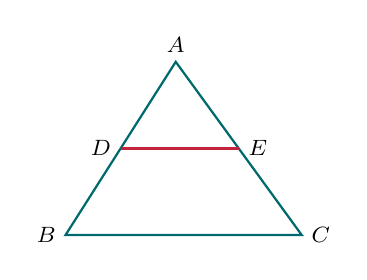
\begin{tikzpicture}[scale=1, font=\fontsize{9.5}{9.5}\selectfont]
  \coordinate (A) at (1.4,2.2); \coordinate (B) at (0,0); \coordinate (C) at (3.0,0);
  \coordinate (D) at ($(A)!0.5!(B)$); \coordinate (E) at ($(A)!0.5!(C)$);
  \draw[thick, color=brandNavy] (A) -- (B) -- (C) -- cycle;
  \draw[thick, color=brandCrimson] (D) -- (E);
  \node[above] at (A) {\footnotesize $A$}; \node[left] at (B) {\footnotesize $B$}; \node[right] at (C) {\footnotesize $C$};
  \node[left] at (D) {\footnotesize $D$}; \node[right] at (E) {\footnotesize $E$};
\end{tikzpicture}
\end{center}

\vspace{1pt}

\exhead{2} គេឱ្យ $\Delta ABC \sim \Delta A'B'C'$ ដែលមានផលធៀបដំណូចស្មើនឹង $k = \dfrac{1}{4}$។ ចូរគណនាតម្លៃនៃ $x, y$ និង $z$ តាមរូបខាងក្រោម ៖
\begin{center}
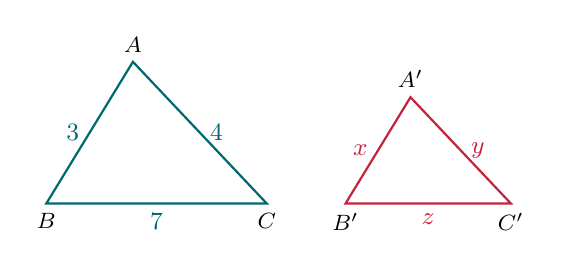
\begin{tikzpicture}[scale=1, font=\fontsize{9.5}{9.5}\selectfont]
  % Triangle ABC
  \coordinate (A) at (1.1,1.8); \coordinate (B) at (0,0); \coordinate (C) at (2.8,0);
  \draw[thick, color=brandNavy] (A) -- node[left]{ $3$} (B) -- node[below]{ $7$} (C) -- node[right]{$4$} cycle;
  \node[above] at (A) {\footnotesize $A$}; \node[below] at (B) {\footnotesize $B$}; \node[below] at (C) {\footnotesize $C$};

  % Triangle A'B'C'
  \begin{scope}[xshift=3.8cm, scale=0.75]
    \coordinate (A1) at (1.1,1.8); \coordinate (B1) at (0,0); \coordinate (C1) at (2.8,0);
    \draw[thick, color=brandCrimson] (A1) -- node[left]{ $x$} (B1) -- node[below]{ $z$} (C1) -- node[right]{ $y$} cycle;
    \node[above] at (A1) {\footnotesize $A'$}; \node[below] at (B1) {\footnotesize $B'$}; \node[below] at (C1) {\footnotesize $C'$};
  \end{scope}
\end{tikzpicture}
\end{center}

\columnbreak

\exhead{3} ក្នុងត្រីកោណ $MNP$ មួយ គេយកចំណុច $S$ និង $T$ នៅលើជ្រុង $MN$ និង $MP$ រៀងគ្នាដែល $ST \parallel NP$ និង $\dfrac{MS}{MN} = \dfrac{1}{3}$។ ចូរបង្ហាញថា $\Delta MST \sim \Delta MNP$ រួចទាញរកផលធៀបដំណូច $k$។
\begin{center}
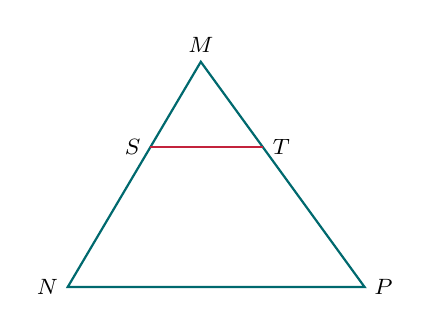
\begin{tikzpicture}[scale=1.3, font=\fontsize{9.5}{9.5}\selectfont]
  \coordinate (M) at (1.3,2.2); \coordinate (N) at (0,0); \coordinate (P) at (2.9,0);
  \coordinate (S) at ($(M)!0.38!(N)$); \coordinate (T) at ($(M)!0.38!(P)$);
  \draw[thick, color=brandNavy] (M) -- (N) -- (P) -- cycle;
  \draw[thick, color=brandCrimson] (S) -- (T);
  \node[above] at (M) {\footnotesize $M$}; \node[left] at (N) {\footnotesize $N$}; \node[right] at (P) {\footnotesize $P$};
  \node[left] at (S) {\footnotesize $S$}; \node[right] at (T) {\footnotesize $T$};
\end{tikzpicture}
\end{center}

\vspace{1pt}

\exhead{4} គេឱ្យ $\Delta DEF \sim \Delta D'E'F'$ ដែលមានផលធៀបដំណូច $k = \dfrac{2}{3}$។ តាមរូបខាងក្រោម ចូរគណនារង្វាស់ជ្រុង $a, b$ និង $c$ ៖
\begin{center}
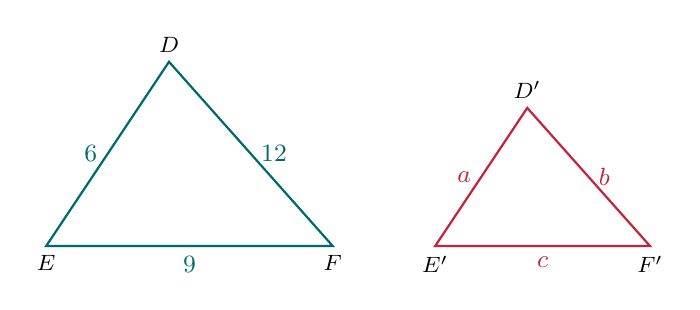
\begin{tikzpicture}[scale=1.3, font=\fontsize{9.5}{9.5}\selectfont]
  % Triangle DEF
  \coordinate (D) at (1.2,1.8); \coordinate (E) at (0,0); \coordinate (F) at (2.8,0);
  \draw[thick, color=brandNavy] (D) -- node[left]{ $6$} (E) -- node[below]{ $9$} (F) -- node[right]{ $12$} cycle;
  \node[above] at (D) {\footnotesize $D$}; \node[below] at (E) {\footnotesize $E$}; \node[below] at (F) {\footnotesize $F$};

  % Triangle D'E'F'
  \begin{scope}[xshift=3.8cm, scale=0.75]
    \coordinate (D1) at (1.2,1.8); \coordinate (E1) at (0,0); \coordinate (F1) at (2.8,0);
    \draw[thick, color=brandCrimson] (D1) -- node[left]{ $a$} (E1) -- node[below]{ $c$} (F1) -- node[right]{ $b$} cycle;
    \node[above] at (D1) {\footnotesize $D'$}; \node[below] at (E1) {\footnotesize $E'$}; \node[below] at (F1) {\footnotesize $F'$};
  \end{scope}
\end{tikzpicture}
\end{center}
\end{multicols}

\vspace{6pt}

\khsubsection{១.២}{ករណីដំណូចទី១ (មុំ-មុំ ៖ ម.ម)}

\begin{khboxorange}
\begin{minipage}[c]{0.56\textwidth}
\textbf{ទ្រឹស្ដីបទ (មុំ-មុំ ៖ ម.ម) ៖} \\
ត្រីកោណពីរជាត្រីកោណដូចគ្នាកាលណាវាមាន\textbf{មុំពីរស្មើគ្នារៀងគ្នា}។
\par\vspace{2pt}
\begin{itemize}[leftmargin=12pt, topsep=0.5pt, itemsep=1pt]
  \item[\color{koreaOrange}\ding{228}] \textbf{លក្ខខណ្ឌ ៖} $\angle A = \angle A' = \alpha$ \quad និង \quad $\angle B = \angle B' = \beta$
  \item[\color{koreaOrange}\ding{228}] \textbf{សន្និដ្ឋាន ៖} \koreahl{$\Delta ABC \sim \Delta A'B'C' \text{ (ម.ម)}$}
  \item[\color{koreaOrange}\ding{228}] \textbf{វិបាក ៖} $\angle C = \angle C'$ \quad និង \quad $\dfrac{AB}{A'B'} = \dfrac{AC}{A'C'} = \dfrac{BC}{B'C'} = k$
\end{itemize}
\end{minipage}\hfill
\begin{minipage}[c]{0.42\textwidth}
\centering
\begin{tikzpicture}[scale=1, font=\fontsize{9.5}{9.5}\selectfont]
  % Triangle ABC
  \coordinate (A) at (1.0, 1.9); \coordinate (B) at (0, 0); \coordinate (C) at (2.6, 0);
  \fill[brandTealBg, opacity=0.5] (A) -- (B) -- (C) -- cycle;
  \draw[thick, color=brandNavy] (A) -- (B) -- (C) -- cycle;
  \node[above] at (A) { $A$}; \node[left] at (B) { $B$}; \node[right] at (C) { $C$};
  \draw[thick, brandCrimson] (A) +(-112:3mm) arc (-112:-38:3mm);
  \node at ($(A)+(0,-0.38)$) { $\alpha$};
  \draw[thick, brandNavy] (B) +(0:3.5mm) arc (0:66:3.5mm);
  \node at ($(B)+(0.48,0.20)$) { $\beta$};

  % Triangle A'B'C'
  \begin{scope}[xshift=3.0cm, yshift=0.15cm, scale=0.62]
    \coordinate (A1) at (1.0, 1.9); \coordinate (B1) at (0, 0); \coordinate (C1) at (2.6, 0);
    \fill[brandGoldBg, opacity=0.5] (A1) -- (B1) -- (C1) -- cycle;
    \draw[thick, color=brandCrimson] (A1) -- (B1) -- (C1) -- cycle;
    \node[above] at (A1) { $A'$}; \node[left] at (B1) { $B'$}; \node[right] at (C1) { $C'$};
    \draw[thick, brandCrimson] (A1) +(-112:3mm) arc (-112:-38:3mm);
    \node at ($(A1)+(0,-0.38)$) { $\alpha$};
    \draw[thick, brandNavy] (B1) +(0:3.5mm) arc (0:66:3.5mm);
    \node at ($(B1)+(0.48,0.20)$) { $\beta$};
  \end{scope}
  \node at (2.3, -0.35) {\fontsize{6.5}{6.5}\selectfont\color{brandCrimson}\textbf{មុំពីរស្មើគ្នារៀងគ្នា $\implies$ (ម.ម)}};
\end{tikzpicture}
\end{minipage}
\end{khboxorange}

\vspace{1pt}

\begin{multicols}{2}
\exhead{1} គេមាន $\Delta ABC$ និង $\Delta DEF$ ដែល $\angle A = 45^\circ, \angle B = 64^\circ, \angle D = 45^\circ, \angle E = 71^\circ$។ ចូរបង្ហាញថា $\Delta ABC \sim \Delta DEF$ រួចទាញរកផលធៀបដំណូច។

\vspace{1pt}

\exhead{2} គេឱ្យ $\angle S = 37^\circ, \angle R = \angle K = 58^\circ$ និង $SR = 72\,\text{m}, SK = 168\,\text{m}, TR = 54\,\text{m}$ ៖
\begin{center}
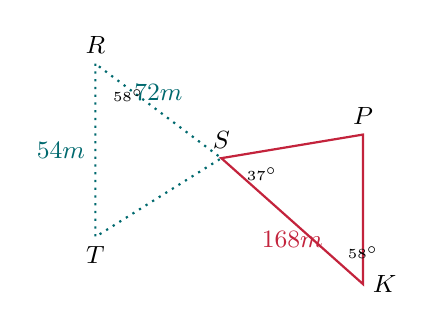
\begin{tikzpicture}[scale=1, font=\fontsize{9.5}{9.5}\selectfont]
  \coordinate (S) at (2.0,1.1);
  \coordinate (R) at (0.4,2.3); \coordinate (T) at (0.4,0.1);
  \coordinate (P) at (3.8,1.4); \coordinate (K) at (3.8,-0.5);
  \draw[thick, dotted, color=brandNavy] (R) -- node[left]{ $54\text{m}$} (T) -- (S) -- node[above]{ $72\text{m}$} cycle;
  \draw[thick, color=brandCrimson] (S) -- (P) -- (K) -- node[below]{ $168\text{m}$} cycle;
  \node[above] at (R) { $R$}; \node[below] at (T) { $T$}; \node[above] at (S) {$S$};
  \node[above] at (P) { $P$}; \node[right] at (K) {$K$};
  \node[below right] at (0.5,2.1) {\fontsize{5}{5}\selectfont $58^\circ$};
  \node[above] at (3.8,-0.3) {\fontsize{5}{5}\selectfont $58^\circ$};
  \node[below right] at (2.2,1.1) {\fontsize{5}{5}\selectfont $37^\circ$};
\end{tikzpicture}
\end{center}
\begin{enumerate}[label=\alph*., leftmargin=12pt, topsep=0.5pt, itemsep=0.5pt]
  \item ចូរបង្ហាញថា $\Delta SPK \sim \Delta STR$
  \item ចូររកប្រវែង $PK$
\end{enumerate}

\columnbreak

\exhead{3} គេមានត្រីកោណ $ABC$ និង $PMN$ ដែល $\angle A = 80^\circ, \angle B = 54^\circ, \angle P = 54^\circ$ និង $\angle M = 46^\circ$ ៖
\begin{enumerate}[label=\alph*., leftmargin=12pt, topsep=0.5pt, itemsep=0.5pt]
  \item ចូរបង្ហាញថាត្រីកោណ $ABC$ ដូចត្រីកោណ $PMN$
  \item ចូរទាញរកផលធៀបដំណូច
\end{enumerate}

\vspace{1pt}

\exhead{4} គេឱ្យបន្ទាត់ $AB \parallel CD$ កាត់គ្នាត្រង់ $O$ ដូចរូបខាងក្រោម។ ចូរបង្ហាញថា $\Delta OAB \sim \Delta OCD$ រួចគណនាប្រវែង $x = CD$ ៖
\begin{center}
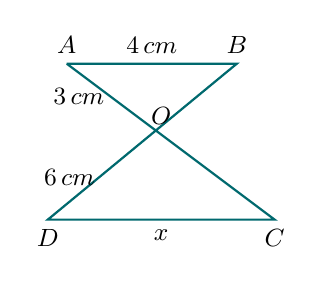
\begin{tikzpicture}[scale=1.2, font=\fontsize{9.5}{9.5}\selectfont]
  \coordinate (A) at (0,1.3); \coordinate (B) at (1.8,1.3);
  \coordinate (O) at (1.0,0.55);
  \coordinate (C) at (2.2,-0.35); \coordinate (D) at (-0.2,-0.35);
  \draw[thick, color=brandNavy] (A) -- (B) -- (D) -- (C) -- (A);
  \node[above] at (A) {$A$}; \node[above] at (B) {$B$};
  \node[above] at (O) { $O$};
  \node[below] at (D) { $D$}; \node[below] at (C) { $C$};
  \node[above] at (0.9,1.3) { $4\,\text{cm}$};
  \node[below] at (1.0,-0.35) { $x$};
  \node[left] at (0.5,0.95) { $3\,\text{cm}$};
  \node[left] at (0.4,0.1) { $6\,\text{cm}$};
\end{tikzpicture}
\end{center}
\end{multicols}

\vspace{2pt}

\khsubsection{១.៣}{ករណីដំណូចទី២ (ជ្រុង-មុំ-ជ្រុង ៖ ជ.ម.ជ)}

\begin{khboxorange}
\begin{minipage}[c]{0.56\textwidth}
\textbf{ទ្រឹស្ដីបទ (ជ្រុង-មុំ-ជ្រុង ៖ ជ.ម.ជ) ៖} \\
ត្រីកោណពីរជាត្រីកោណដូចគ្នាកាលណាវាមាន\textbf{មុំមួយប៉ុនរៀងគ្នា អមដោយជ្រុងពីរមានផលធៀបសមាមាត្ររៀងគ្នា}។
\par\vspace{2pt}
\begin{itemize}[leftmargin=12pt, topsep=0.5pt, itemsep=1pt]
  \item[\color{koreaOrange}\ding{228}] \textbf{លក្ខខណ្ឌ ៖} $\angle A = \angle A'$ \quad និង \quad $\dfrac{AB}{A'B'} = \dfrac{AC}{A'C'} = k$
  \item[\color{koreaOrange}\ding{228}] \textbf{សន្និដ្ឋាន ៖} \koreahl{$\Delta ABC \sim \Delta A'B'C' \text{ (ជ.ម.ជ)}$}
  \item[\color{koreaOrange}\ding{228}] \textbf{វិបាក ៖} $\angle B = \angle B', \ \angle C = \angle C'$ \quad និង \quad $\dfrac{BC}{B'C'} = k$
\end{itemize}
\end{minipage}\hfill
\begin{minipage}[c]{0.42\textwidth}
\centering
\begin{tikzpicture}[scale=1.2, font=\fontsize{9.5}{9.5}\selectfont]
  % Triangle ABC
  \coordinate (A) at (1.0, 1.9); \coordinate (B) at (0, 0); \coordinate (C) at (2.5, 0);
  \fill[brandTealBg, opacity=0.5] (A) -- (B) -- (C) -- cycle;
  \draw[line width=1.2pt, color=brandNavy] (B) -- (A) -- (C);
  \draw[thick, dashed, color=brandNavy!60] (B) -- (C);
  \node[above] at (A) { $A$}; \node[left] at (B) { $B$}; \node[right] at (C) { $C$};
  \draw[thick, brandCrimson] (A) +(-112:3mm) arc (-112:-38:3mm);
  \node at ($(A)+(0,-0.38)$) {$\alpha$};
  \node[left] at ($(A)!0.5!(B)$) { $c$}; \node[right] at ($(A)!0.5!(C)$) { $b$};

  % Triangle A'B'C'
  \begin{scope}[xshift=2.9cm, yshift=0.15cm, scale=0.60]
    \coordinate (A1) at (1.0, 1.9); \coordinate (B1) at (0, 0); \coordinate (C1) at (2.5, 0);
    \fill[brandGoldBg, opacity=0.5] (A1) -- (B1) -- (C1) -- cycle;
    \draw[line width=1.2pt, color=brandCrimson] (B1) -- (A1) -- (C1);
    \draw[thick, dashed, color=brandCrimson!60] (B1) -- (C1);
    \node[above] at (A1) { $A'$}; \node[left] at (B1) {$B'$}; \node[right] at (C1) { $C'$};
    \draw[thick, brandCrimson] (A1) +(-112:3mm) arc (-112:-38:3mm);
    \node at ($(A1)+(0,-0.38)$) { $\alpha$};
    \node[left] at ($(A1)!0.5!(B1)$) { $kc$}; \node[right] at ($(A1)!0.5!(C1)$) { $kb$};
  \end{scope}
  \node at (2.3, -0.35) {\fontsize{7.5}{6.5}\selectfont\color{brandCrimson}\textbf{មុំមួយ និងជ្រុងអមសមាមាត្រ $\implies$ (ជ.ម.ជ)}};
\end{tikzpicture}
\end{minipage}
\end{khboxorange}

\vspace{1.5pt}

\begin{multicols}{2}
\exhead{1} គេមានបន្ទាត់ $PH$ និង $FM$ កែងគ្នាត្រង់ $H$ ដែល $FH = 2HM$ និងចំណុច $N$ កណ្ដាលនៃ $PH$ ។ ចូរស្រាយបញ្ជាក់ថា $\Delta PHF \sim \Delta NHM$ ។

\vspace{1.5pt}

\exhead{2} គេមាន $\Delta ABC \sim \Delta AEF$ តាមរូបខាងក្រោម ។ ចូរគណនាប្រវែងជ្រុង $AE$ និង $AF$ ៖
\begin{center}
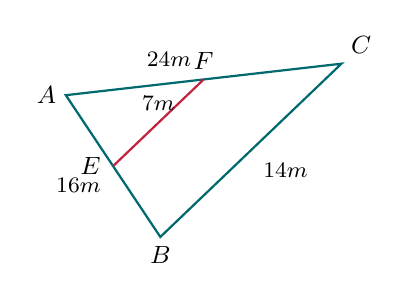
\begin{tikzpicture}[scale=1, font=\fontsize{9.5}{9.5}\selectfont]
  \coordinate (A) at (0, 1.4);
  \coordinate (B) at (1.2, -0.4);
  \coordinate (C) at (3.5, 1.8);
  \coordinate (E) at ($(A)!0.5!(B)$);
  \coordinate (F) at ($(A)!0.5!(C)$);

  \draw[thick, color=brandNavy] (A) -- (B) -- (C) -- cycle;
  \draw[thick, color=brandCrimson] (E) -- (F);

  \node[left] at (A) { $A$};
  \node[below] at (B) { $B$};
  \node[above right] at (C) { $C$};
  \node[left=1pt] at (E) { $E$};
  \node[above] at (F) { $F$};

  \node[above left=1pt] at ($(A)!0.5!(C)$) {\fontsize{8.5}{8.5}\selectfont $24\text{m}$};
  \node[below left=1pt] at ($(A)!0.5!(B)$) {\fontsize{8.5}{8.5}\selectfont $16\text{m}$};
  \node[below right=1pt] at ($(B)!0.5!(C)$) {\fontsize{8.5}{8.5}\selectfont $14\text{m}$};
  \node[above=1pt] at ($(E)!0.5!(F)$) {\fontsize{8.5}{8.5}\selectfont $7\text{m}$};
\end{tikzpicture}
\end{center}

\columnbreak

\exhead{3} ចូរគណនាប្រវែងទទឹងនៃទន្លេ $AB$ តាមរូបខាងក្រោម ដោយត្រីកោណ $CBA$ ដូចត្រីកោណ $CDE$ ៖
\begin{center}
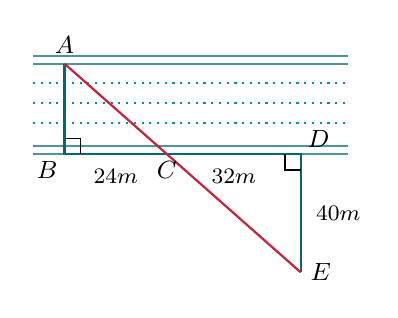
\begin{tikzpicture}[scale=1, font=\fontsize{9.5}{9.5}\selectfont]
  % River banks
  \draw[thick, color=brandNavy!70] (-0.4, 1.4) -- (3.6, 1.4);
  \draw[thick, color=brandNavy!70] (-0.4, 1.3) -- (3.6, 1.3);
  
  \draw[dotted, color=brandTeal, thick] (-0.4, 1.05) -- (3.6, 1.05);
  \draw[dotted, color=brandTeal, thick] (-0.4, 0.8) -- (3.6, 0.8);
  \draw[dotted, color=brandTeal, thick] (-0.4, 0.55) -- (3.6, 0.55);
  
  \draw[thick, color=brandNavy!70] (-0.4, 0.25) -- (3.6, 0.25);
  \draw[thick, color=brandNavy!70] (-0.4, 0.15) -- (3.6, 0.15);

  % Geometric vertices
  \coordinate (A) at (0, 1.3);
  \coordinate (B) at (0, 0.15);
  \coordinate (C) at (1.3, 0.15);
  \coordinate (D) at (3.0, 0.15);
  \coordinate (E) at (3.0, -1.35);

  % River crossing line and boundary lines
  \draw[thick, color=brandNavy] (A) -- (B) -- (D) -- (E);
  \draw[thick, color=brandCrimson] (A) -- (E);

  % Right angle marks
  \draw[thin] (0, 0.35) -- (0.2, 0.35) -- (0.2, 0.15);
  \draw[thin] (3.0, -0.05) -- (2.8, -0.05) -- (2.8, 0.15);

  % Labels
  \node[above] at (A) { $A$};
  \node[below left=-1pt] at (B) {$B$};
  \node[below=-1pt] at (C) {$C$};
  \node[above right=-1pt] at (D) { $D$};
  \node[right] at (E) { $E$};

  \node[below=2pt] at ($(B)!0.5!(C)$) {\fontsize{8.5}{8.5}\selectfont $24\text{m}$};
  \node[below=2pt] at ($(C)!0.5!(D)$) {\fontsize{8.5}{8.5}\selectfont $32\text{m}$};
  \node[right=2pt] at ($(D)!0.5!(E)$) {\fontsize{8.5}{8.5}\selectfont $40\text{m}$};
\end{tikzpicture}
\end{center}
\end{multicols}

\vspace{2pt}

% #########################################################################
% PAGE 3: ផ្នែកទី ១ (ត) ៖ ករណីដំណូចទី៣ (ជ.ជ.ជ) & តារាងប្រៀបធៀបសង្ខេប
% #########################################################################
\khsubsection{១.៤}{ករណីដំណូចទី៣ (ជ្រុង-ជ្រុង-ជ្រុង ៖ ជ.ជ.ជ)}

\begin{khboxorange}[top=2pt, bottom=2pt, left=6pt, right=6pt]
\begin{minipage}[c]{0.58\textwidth}
\textbf{ទ្រឹស្ដីបទ (ជ្រុង-ជ្រុង-ជ្រុង ៖ ជ.ជ.ជ) ៖} \\
ត្រីកោណពីរជាត្រីកោណដូចគ្នាកាលណាវាមាន \textbf{ជ្រុងទាំងបីសមាមាត្ររៀងគ្នា}។
\par\vspace{1pt}
\begin{itemize}[leftmargin=12pt, topsep=0pt, itemsep=0.5pt]
  \item[\color{koreaOrange}\ding{228}] \textbf{លក្ខខណ្ឌ ៖} $\dfrac{AB}{A'B'} = \dfrac{AC}{A'C'} = \dfrac{BC}{B'C'} = k$
  \item[\color{koreaOrange}\ding{228}] \textbf{សន្និដ្ឋាន ៖} \koreahl{$\Delta ABC \sim \Delta A'B'C' \text{ (ជ.ជ.ជ)}$}
  \item[\color{koreaOrange}\ding{228}] \textbf{វិបាក ៖} $\angle A = \angle A', \ \angle B = \angle B', \ \angle C = \angle C'$
\end{itemize}
\end{minipage}\hfill
\begin{minipage}[c]{0.40\textwidth}
\centering
\begin{tikzpicture}[scale=0.75, font=\fontsize{8.5}{8.5}\selectfont]
  % Triangle ABC
  \coordinate (A) at (1.0, 1.6); \coordinate (B) at (0, 0); \coordinate (C) at (2.4, 0);
  \fill[brandTealBg, opacity=0.5] (A) -- (B) -- (C) -- cycle;
  \draw[line width=1.1pt, color=brandNavy] (A) -- (B) -- (C) -- cycle;
  \node[above] at (A) {$A$}; \node[left] at (B) {$B$}; \node[right] at (C) {$C$};
  \node[left] at ($(A)!0.5!(B)$) {$c$}; \node[below] at ($(B)!0.5!(C)$) {$a$}; \node[right] at ($(A)!0.5!(C)$) {$b$};

  % Triangle A'B'C'
  \begin{scope}[xshift=2.7cm, yshift=0.1cm, scale=0.60]
    \coordinate (A1) at (1.0, 1.6); \coordinate (B1) at (0, 0); \coordinate (C1) at (2.4, 0);
    \fill[brandGoldBg, opacity=0.5] (A1) -- (B1) -- (C1) -- cycle;
    \draw[line width=1.1pt, color=brandCrimson] (A1) -- (B1) -- (C1) -- cycle;
    \node[above] at (A1) {$A'$}; \node[left] at (B1) {$B'$}; \node[right] at (C1) {$C'$};
    \node[left] at ($(A1)!0.5!(B1)$) {$kc$}; \node[below] at ($(B1)!0.5!(C1)$) {$ka$}; \node[right] at ($(A1)!0.5!(C1)$) {$kb$};
  \end{scope}
  \node at (2.2, -0.32) {\fontsize{6.5}{6.5}\selectfont\color{brandCrimson}\textbf{ជ្រុងទាំងបីសមាមាត្រ $\implies$ (ជ.ជ.ជ)}};
\end{tikzpicture}
\end{minipage}
\end{khboxorange}

\vspace{1pt}

\begin{multicols}{2}
\exhead{1} គេមានត្រីកោណ $ABC$ ដែល $AB=15, BC=21, AC=9$ ហើយត្រីកោណ $XYZ$ មួយទៀតមាន $XY=5, YZ=7, XZ=3$។ បង្ហាញថាត្រីកោណ $ABC$ និង $XYZ$ ជាត្រីកោណដូចគ្នា រួចទាញរកវិបាក។

\vspace{1pt}

\exhead{2} គេឱ្យត្រីកោណពីរដូចរូបខាងក្រោម ៖
\begin{center}\vspace{-6pt}
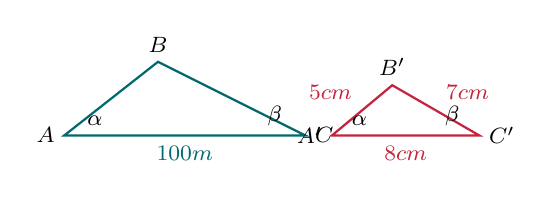
\begin{tikzpicture}[scale=0.85, font=\fontsize{8.5}{8.5}\selectfont]
  \coordinate (A) at (0,0); \coordinate (B) at (1.4,1.1); \coordinate (C) at (3.6,0);
  \draw[thick, color=brandNavy] (A) -- (B) -- (C) -- node[below]{$100\text{m}$} cycle;
  \node[left] at (A) {$A$}; \node[above] at (B) {$B$}; \node[right] at (C) {$C$};
  \node[above right] at (0.2,0) {$\alpha$}; \node[above left] at (3.4,0) {$\beta$};

  \begin{scope}[xshift=4.0cm]
    \coordinate (A1) at (0,0); \coordinate (B1) at (0.9,0.75); \coordinate (C1) at (2.2,0);
    \draw[thick, color=brandCrimson] (A1) -- node[above left]{$5\text{cm}$} (B1) -- node[above right]{$7\text{cm}$} (C1) -- node[below]{$8\text{cm}$} cycle;
    \node[left] at (A1) {$A'$}; \node[above] at (B1) {$B'$}; \node[right] at (C1) {$C'$};
    \node[above right] at (0.15,0) {$\alpha$}; \node[above left] at (2.05,0) {$\beta$};
  \end{scope}
\end{tikzpicture}
\vspace{-6pt}\end{center}
\begin{enumerate}[label=\alph*., leftmargin=12pt, topsep=0pt, itemsep=0.5pt]
  \item ប្រដូចត្រីកោណ $ABC$ និង $A'B'C'$
  \item ចូរគណនាប្រវែង $AB$ និង $BC$
\end{enumerate}

\vspace{1pt}

\exhead{3} ចូរគណនាប្រវែងជ្រុង $AC$ នៃត្រីកោណកែង $ABC$ តាមរូបខាងក្រោម ៖
\begin{center}\vspace{-6pt}
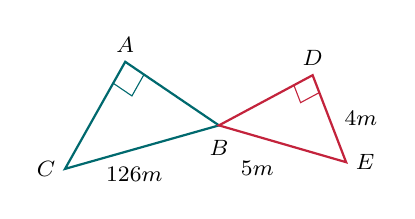
\begin{tikzpicture}[scale=0.85, font=\fontsize{8.5}{8.5}\selectfont]
  \coordinate (B) at (0, 0);
  \coordinate (A) at (-1.4, 0.95);
  \coordinate (C) at (-2.3, -0.65);
  \coordinate (D) at (1.4, 0.75);
  \coordinate (E) at (1.9, -0.55);

  \draw[thick, color=brandNavy] (C) -- (A) -- (B) -- cycle;
  \draw[thick, color=brandCrimson] (B) -- (D) -- (E) -- cycle;

  % Right angle marks
  \coordinate (a1) at ($(A)!0.2!(C)$);
  \coordinate (a2) at ($(A)!0.2!(B)$);
  \draw[thin, color=brandNavy] (a1) -- ($(a1)+(a2)-(A)$) -- (a2);

  \coordinate (d1) at ($(D)!0.2!(B)$);
  \coordinate (d2) at ($(D)!0.2!(E)$);
  \draw[thin, color=brandCrimson] (d1) -- ($(d1)+(d2)-(D)$) -- (d2);

  \node[left] at (C) {$C$};
  \node[above] at (A) {$A$};
  \node[below=2pt] at (B) {$B$};
  \node[above] at (D) {$D$};
  \node[right] at (E) {$E$};

  \node[below=3pt] at ($(C)!0.45!(B)$) {\fontsize{8}{8}\selectfont $126\text{m}$};
  \node[below left=2pt] at ($(B)!0.55!(E)$) {\fontsize{8}{8}\selectfont $5\text{m}$};
  \node[right=2pt] at ($(D)!0.5!(E)$) {\fontsize{8}{8}\selectfont $4\text{m}$};
\end{tikzpicture}
\vspace{-6pt}\end{center}

\columnbreak

\exhead{4} ចូរគណនាតម្លៃ $x$ និង $y$ តាមរូបនីមួយៗខាងក្រោម ៖
\par\vspace{1pt}
\noindent\begin{minipage}[t]{0.48\linewidth}
\centering
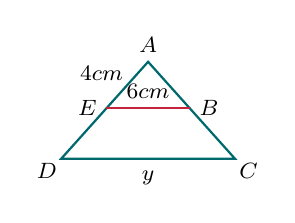
\begin{tikzpicture}[scale=0.85, font=\fontsize{8.5}{8.5}\selectfont]
  \coordinate (A) at (1.3, 1.45);
  \coordinate (D) at (0, 0);
  \coordinate (C) at (2.6, 0);
  \coordinate (E) at ($(A)!0.48!(D)$);
  \coordinate (B) at ($(A)!0.48!(C)$);
  \draw[thick, color=brandNavy] (A) -- (D) -- (C) -- cycle;
  \draw[thick, color=brandCrimson] (E) -- (B);
  \node[above] at (A) {$A$};
  \node[below left=-2pt] at (D) {$D$};
  \node[below right=-2pt] at (C) {$C$};
  \node[left=0pt] at (E) {$E$};
  \node[right=0pt] at (B) {$B$};
  \node[above=0pt] at ($(E)!0.5!(B)$) {\fontsize{8}{8}\selectfont $6\text{cm}$};
  \node[below=1pt] at ($(D)!0.5!(C)$) {\fontsize{8}{8}\selectfont $y$};
  \node[above left=-2pt] at ($(A)!0.5!(E)$) {\fontsize{8}{8}\selectfont $4\text{cm}$};
\end{tikzpicture}\\[1pt]
{\fontsize{8}{9}\selectfont\textbf{ក.} $AE{=}4\text{cm}, AD{=}10\text{cm}$}
\end{minipage}\hfill
\begin{minipage}[t]{0.48\linewidth}
\centering
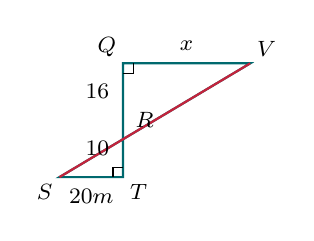
\begin{tikzpicture}[scale=0.85, font=\fontsize{8.5}{8.5}\selectfont]
  \coordinate (Q) at (0, 1.25);
  \coordinate (V) at (1.9, 1.25);
  \coordinate (R) at (0, 0.4);
  \coordinate (T) at (0, -0.45);
  \coordinate (S) at (-0.95, -0.45);
  \draw[thick, color=brandNavy] (V) -- (Q) -- (T) -- (S) -- cycle;
  \draw[thick, color=brandCrimson] (V) -- (S);
  \draw[thin] (0, 1.1) -- (0.15, 1.1) -- (0.15, 1.25);
  \draw[thin] (0, -0.3) -- (-0.15, -0.3) -- (-0.15, -0.45);
  \node[above left=-1pt] at (Q) {$Q$};
  \node[above right=-1pt] at (V) {$V$};
  \node[right=1pt] at (0, 0.4) {$R$};
  \node[below right=-1pt] at (T) {$T$};
  \node[below left=-1pt] at (S) {$S$};
  \node[above=1pt] at ($(Q)!0.5!(V)$) {\fontsize{8}{8}\selectfont $x$};
  \node[below=1pt] at ($(S)!0.5!(T)$) {\fontsize{8}{8}\selectfont $20\text{m}$};
  \node[left=1.5pt] at ($(Q)!0.5!(R)$) {\fontsize{8}{8}\selectfont $16$};
  \node[left=1.5pt] at ($(R)!0.5!(T)$) {\fontsize{8}{8}\selectfont $10$};
\end{tikzpicture}\\[1pt]
{\fontsize{8}{9}\selectfont\textbf{ខ.} $QR{=}16\text{cm}, RT{=}10\text{cm}$}
\end{minipage}

\vspace{1pt}

\exhead{5} ចូរគណនាតម្លៃ $x$ តាមរូបនីមួយៗខាងក្រោម ៖
\par\vspace{1pt}
\noindent\begin{minipage}[t]{0.48\linewidth}
\centering
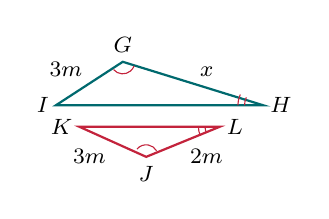
\begin{tikzpicture}[scale=0.85, font=\fontsize{8.5}{8.5}\selectfont]
  % Triangle GHI
  \coordinate (I) at (0, 0);
  \coordinate (G) at (1.0, 0.65);
  \coordinate (H) at (3.1, 0);
  \draw[thick, color=brandNavy] (I) -- (G) -- (H) -- cycle;
  \draw[color=brandCrimson] ($(G)+(-140:0.18)$) arc (-140:-20:0.18);
  \draw[color=brandCrimson] ($(H)+(180:0.28)$) arc (180:155:0.28);
  \draw[color=brandCrimson] ($(H)+(180:0.38)$) arc (180:155:0.38);
  \node[left=-1pt] at (I) {$I$};
  \node[above] at (G) {$G$};
  \node[right=-1pt] at (H) {$H$};
  \node[above left=-1pt] at ($(I)!0.5!(G)$) {\fontsize{8}{8}\selectfont $3\text{m}$};
  \node[above right=-1pt] at ($(G)!0.5!(H)$) {\fontsize{8}{8}\selectfont $x$};

  % Triangle JKL below
  \begin{scope}[yshift=-0.32cm]
    \coordinate (K) at (0.35, 0);
    \coordinate (J) at (1.35, -0.45);
    \coordinate (L) at (2.45, 0);
    \draw[thick, color=brandCrimson] (K) -- (J) -- (L) -- cycle;
    \draw[color=brandCrimson] ($(J)+(140:0.18)$) arc (140:30:0.18);
    \draw[color=brandCrimson] ($(L)+(180:0.22)$) arc (180:205:0.22);
    \draw[color=brandCrimson] ($(L)+(180:0.32)$) arc (180:205:0.32);
    \node[left=-1pt] at (K) {$K$};
    \node[below] at (J) {$J$};
    \node[right=-1pt] at (L) {$L$};
    \node[below left=-1pt] at ($(K)!0.5!(J)$) {\fontsize{8}{8}\selectfont $3\text{m}$};
    \node[below right=-1pt] at ($(J)!0.5!(L)$) {\fontsize{8}{8}\selectfont $2\text{m}$};
  \end{scope}
\end{tikzpicture}\\[1pt]
{\fontsize{8}{9}\selectfont\textbf{គ.} $\Delta GHI \sim \Delta JKL$}
\end{minipage}\hfill
\begin{minipage}[t]{0.48\linewidth}
\centering
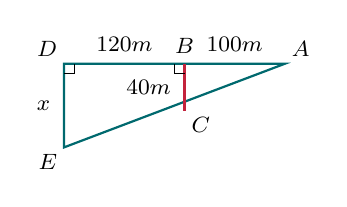
\begin{tikzpicture}[scale=0.85, font=\fontsize{8.5}{8.5}\selectfont]
  \coordinate (A) at (3.3, 1.25);
  \coordinate (B) at (1.8, 1.25);
  \coordinate (D) at (0, 1.25);
  \coordinate (C) at (1.8, 0.55);
  \coordinate (E) at (0, 0);
  
  \draw[thick, color=brandNavy] (D) -- (A) -- (E) -- cycle;
  \draw[thick, color=brandCrimson] (B) -- (C);

  % Right angle marks
  \draw[thin] (1.8, 1.1) -- (1.65, 1.1) -- (1.65, 1.25);
  \draw[thin] (0, 1.1) -- (0.15, 1.1) -- (0.15, 1.25);

  \node[above left=-1pt] at (D) {$D$};
  \node[above] at (B) {$B$};
  \node[above right=-1pt] at (A) {$A$};
  \node[below right=-1pt] at (C) {$C$};
  \node[below left=-1pt] at (E) {$E$};

  \node[above=1pt] at ($(D)!0.5!(B)$) {\fontsize{8}{8}\selectfont $120\text{m}$};
  \node[above=1pt] at ($(B)!0.5!(A)$) {\fontsize{8}{8}\selectfont $100\text{m}$};
  \node[left=1.5pt] at ($(B)!0.5!(C)$) {\fontsize{8}{8}\selectfont $40\text{m}$};
  \node[left=1.5pt] at ($(D)!0.5!(E)$) {\fontsize{8}{8}\selectfont $x$};
\end{tikzpicture}\\[1pt]
{\fontsize{8}{9}\selectfont\textbf{ឃ.} $BC \parallel DE$}
\end{minipage}
\end{multicols}

\vspace{-2pt}

\begin{khcard}[top=2pt, bottom=2pt, left=4pt, right=4pt]
\noindent{\fontsize{9.5}{9.5}\selectfont\kml\color{brandCrimson}\textbf{\ding{45}\ ចំណាំ ៖ តារាងប្រៀបធៀបករណីប៉ុនគ្នានៃត្រីកោណ និង ករណីដំណូចនៃត្រីកោណ}}
\par\vspace{1.5pt}
\centering
\renewcommand{\arraystretch}{1.05}
\fontsize{8}{9}\selectfont
\begin{tabular}{|m{7.2cm}|c|c|m{7.2cm}|}
\hline
\multicolumn{2}{|c|}{\cellcolor{brandLightBlue}\textbf{\color{brandNavy}\small លក្ខខណ្ឌនៃត្រីកោណពីរប៉ុនគ្នា}} & \multicolumn{2}{c|}{\cellcolor{brandTealBg}\textbf{\color{brandNavy}\small លក្ខខណ្ឌនៃត្រីកោណពីរដូចគ្នា}} \\ \hline
\cellcolor{brandLightBlue}\centering\textbf{\color{brandNavy}លក្ខណៈ} & \cellcolor{brandLightBlue}\centering\textbf{\color{brandNavy}ករណី} & \cellcolor{brandTealBg}\centering\textbf{\color{brandNavy}ករណី} & \cellcolor{brandTealBg}\centering\textbf{\color{brandNavy}លក្ខណៈ} \tabularnewline \hline

% Row 1: ASA vs AA
\begin{minipage}[c]{7.0cm}
\centering\vspace{1pt}
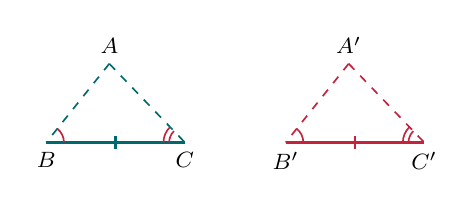
\begin{tikzpicture}[scale=0.8, font=\fontsize{8.5}{8.5}\selectfont]
  % Congruent 1
  \coordinate (A) at (1.0, 1.25); \coordinate (B) at (0, 0); \coordinate (C) at (2.2, 0);
  \draw[dashed, line width=0.6pt, color=brandNavy] (A) -- (B); 
  \draw[dashed, line width=0.6pt, color=brandNavy] (A) -- (C);
  \draw[thick, color=brandNavy] (B) -- (C);
  \node[above] at (A) {\footnotesize $A$}; \node[below] at (B) {\footnotesize $B$}; \node[below] at (C) {\footnotesize $C$};
  \draw[color=brandCrimson, line width=0.6pt] ($(B)+(0:0.28)$) arc (0:52:0.28);
  \draw[color=brandCrimson, line width=0.6pt] ($(C)+(180:0.25)$) arc (180:134:0.25);
  \draw[color=brandCrimson, line width=0.6pt] ($(C)+(180:0.34)$) arc (180:134:0.34);
  \draw[thick, color=brandNavy] (1.10,-0.10) -- (1.10,0.10);

  % Congruent 2
  \begin{scope}[xshift=3.8cm]
    \coordinate (A1) at (1.0, 1.25); \coordinate (B1) at (0, 0); \coordinate (C1) at (2.2, 0);
    \draw[dashed, line width=0.6pt, color=brandCrimson] (A1) -- (B1); 
    \draw[dashed, line width=0.6pt, color=brandCrimson] (A1) -- (C1);
    \draw[thick, color=brandCrimson] (B1) -- (C1);
    \node[above] at (A1) {\footnotesize $A'$}; \node[below] at (B1) {\footnotesize $B'$}; \node[below] at (C1) {\footnotesize $C'$};
    \draw[color=brandCrimson, line width=0.6pt] ($(B1)+(0:0.28)$) arc (0:52:0.28);
    \draw[color=brandCrimson, line width=0.6pt] ($(C1)+(180:0.25)$) arc (180:134:0.25);
    \draw[color=brandCrimson, line width=0.6pt] ($(C1)+(180:0.34)$) arc (180:134:0.34);
    \draw[thick, color=brandCrimson] (1.10,-0.10) -- (1.10,0.10);
  \end{scope}
\end{tikzpicture}\\[0pt]
{\fontsize{7.5}{8.5}\selectfont $\angle B = \angle B', \quad \angle C = \angle C', \quad BC = B'C'$}
\vspace{1pt}
\end{minipage}
& \begin{tabular}{c}\textbf{ទី ១} \\ \textbf{ម.ជ.ម}\end{tabular}
& \begin{tabular}{c}\textbf{ទី ១} \\ \textbf{ម.ម}\end{tabular}
& \begin{minipage}[c]{7.0cm}
\centering\vspace{1pt}
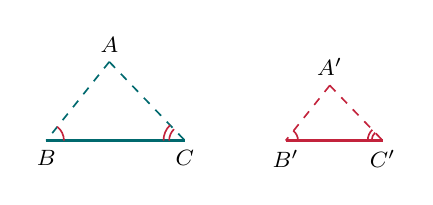
\begin{tikzpicture}[scale=0.8, font=\fontsize{8.5}{8.5}\selectfont]
  % Similar 1
  \coordinate (A) at (1.0, 1.25); \coordinate (B) at (0, 0); \coordinate (C) at (2.2, 0);
  \draw[dashed, line width=0.6pt, color=brandNavy] (A) -- (B); 
  \draw[dashed, line width=0.6pt, color=brandNavy] (A) -- (C);
  \draw[thick, color=brandNavy] (B) -- (C);
  \node[above] at (A) {\footnotesize $A$}; \node[below] at (B) {\footnotesize $B$}; \node[below] at (C) {\footnotesize $C$};
  \draw[color=brandCrimson, line width=0.6pt] ($(B)+(0:0.28)$) arc (0:52:0.28);
  \draw[color=brandCrimson, line width=0.6pt] ($(C)+(180:0.25)$) arc (180:134:0.25);
  \draw[color=brandCrimson, line width=0.6pt] ($(C)+(180:0.34)$) arc (180:134:0.34);

  % Similar 2 (smaller)
  \begin{scope}[xshift=3.8cm, scale=0.70]
    \coordinate (A1) at (1.0, 1.25); \coordinate (B1) at (0, 0); \coordinate (C1) at (2.2, 0);
    \draw[dashed, line width=0.6pt, color=brandCrimson] (A1) -- (B1); 
    \draw[dashed, line width=0.6pt, color=brandCrimson] (A1) -- (C1);
    \draw[thick, color=brandCrimson] (B1) -- (C1);
    \node[above] at (A1) {\footnotesize $A'$}; \node[below] at (B1) {\footnotesize $B'$}; \node[below] at (C1) {\footnotesize $C'$};
    \draw[color=brandCrimson, line width=0.6pt] ($(B1)+(0:0.28)$) arc (0:52:0.28);
    \draw[color=brandCrimson, line width=0.6pt] ($(C1)+(180:0.25)$) arc (180:134:0.25);
    \draw[color=brandCrimson, line width=0.6pt] ($(C1)+(180:0.34)$) arc (180:134:0.34);
  \end{scope}
\end{tikzpicture}\\[0pt]
{\fontsize{7.5}{8.5}\selectfont $\angle B = \angle B', \quad \angle C = \angle C'$}
\vspace{1pt}
\end{minipage} \tabularnewline \hline

% Row 2: SAS vs SAS
\begin{minipage}[c]{7.0cm}
\centering\vspace{1pt}
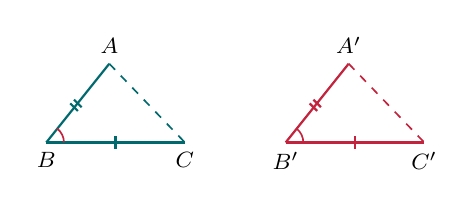
\begin{tikzpicture}[scale=0.8, font=\fontsize{8.5}{8.5}\selectfont]
  % Congruent 1
  \coordinate (A) at (1.0, 1.25); \coordinate (B) at (0, 0); \coordinate (C) at (2.2, 0);
  \draw[thick, color=brandNavy] (A) -- (B); \draw[thick, color=brandNavy] (B) -- (C);
  \draw[dashed, line width=0.6pt, color=brandNavy] (A) -- (C);
  \node[above] at (A) {\footnotesize $A$}; \node[below] at (B) {\footnotesize $B$}; \node[below] at (C) {\footnotesize $C$};
  \draw[color=brandCrimson, line width=0.6pt] ($(B)+(0:0.28)$) arc (0:52:0.28);
  \draw[thick, color=brandNavy] (0.38,0.62) -- (0.50,0.50); \draw[thick, color=brandNavy] (0.44,0.68) -- (0.56,0.56);
  \draw[thick, color=brandNavy] (1.10,-0.10) -- (1.10,0.10);

  % Congruent 2
  \begin{scope}[xshift=3.8cm]
    \coordinate (A1) at (1.0, 1.25); \coordinate (B1) at (0, 0); \coordinate (C1) at (2.2, 0);
    \draw[thick, color=brandCrimson] (A1) -- (B1); \draw[thick, color=brandCrimson] (B1) -- (C1);
    \draw[dashed, line width=0.6pt, color=brandCrimson] (A1) -- (C1);
    \node[above] at (A1) {\footnotesize $A'$}; \node[below] at (B1) {\footnotesize $B'$}; \node[below] at (C1) {\footnotesize $C'$};
    \draw[color=brandCrimson, line width=0.6pt] ($(B1)+(0:0.28)$) arc (0:52:0.28);
    \draw[thick, color=brandCrimson] (0.38,0.62) -- (0.50,0.50); \draw[thick, color=brandCrimson] (0.44,0.68) -- (0.56,0.56);
    \draw[thick, color=brandCrimson] (1.10,-0.10) -- (1.10,0.10);
  \end{scope}
\end{tikzpicture}\\[0pt]
{\fontsize{7.5}{8.5}\selectfont $\angle B = \angle B', \quad AB = A'B', \quad BC = B'C'$}
\vspace{1pt}
\end{minipage}
& \begin{tabular}{c}\textbf{ទី ២} \\ \textbf{ជ.ម.ជ}\end{tabular}
& \begin{tabular}{c}\textbf{ទី ២} \\ \textbf{ជ.ម.ជ}\end{tabular}
& \begin{minipage}[c]{7.0cm}
\centering\vspace{1pt}
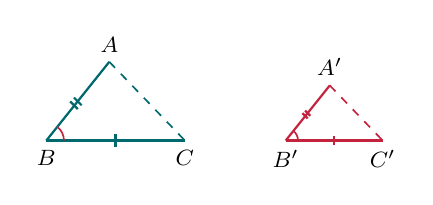
\begin{tikzpicture}[scale=0.8, font=\fontsize{8.5}{8.5}\selectfont]
  % Similar 1
  \coordinate (A) at (1.0, 1.25); \coordinate (B) at (0, 0); \coordinate (C) at (2.2, 0);
  \draw[thick, color=brandNavy] (A) -- (B); \draw[thick, color=brandNavy] (B) -- (C);
  \draw[dashed, line width=0.6pt, color=brandNavy] (A) -- (C);
  \node[above] at (A) {\footnotesize $A$}; \node[below] at (B) {\footnotesize $B$}; \node[below] at (C) {\footnotesize $C$};
  \draw[color=brandCrimson, line width=0.6pt] ($(B)+(0:0.28)$) arc (0:52:0.28);
  \draw[thick, color=brandNavy] (0.38,0.62) -- (0.50,0.50); \draw[thick, color=brandNavy] (0.44,0.68) -- (0.56,0.56);
  \draw[thick, color=brandNavy] (1.10,-0.10) -- (1.10,0.10);

  % Similar 2 (smaller)
  \begin{scope}[xshift=3.8cm, scale=0.70]
    \coordinate (A1) at (1.0, 1.25); \coordinate (B1) at (0, 0); \coordinate (C1) at (2.2, 0);
    \draw[thick, color=brandCrimson] (A1) -- (B1); \draw[thick, color=brandCrimson] (B1) -- (C1);
    \draw[dashed, line width=0.6pt, color=brandCrimson] (A1) -- (C1);
    \node[above] at (A1) {\footnotesize $A'$}; \node[below] at (B1) {\footnotesize $B'$}; \node[below] at (C1) {\footnotesize $C'$};
    \draw[color=brandCrimson, line width=0.6pt] ($(B1)+(0:0.28)$) arc (0:52:0.28);
    \draw[thick, color=brandCrimson] (0.38,0.62) -- (0.50,0.50); \draw[thick, color=brandCrimson] (0.44,0.68) -- (0.56,0.56);
    \draw[thick, color=brandCrimson] (1.10,-0.10) -- (1.10,0.10);
  \end{scope}
\end{tikzpicture}\\[0pt]
{\fontsize{7.5}{8.5}\selectfont $\angle B = \angle B', \quad \dfrac{AB}{A'B'} = \dfrac{BC}{B'C'}$}
\vspace{1pt}
\end{minipage} \tabularnewline \hline

% Row 3: SSS vs SSS
\begin{minipage}[c]{7.0cm}
\centering\vspace{3pt}
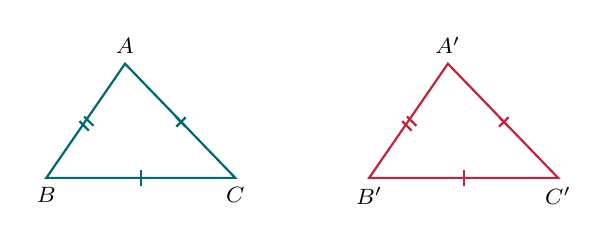
\begin{tikzpicture}[scale=1, font=\fontsize{9.5}{9.5}\selectfont]
  % Congruent 1
  \coordinate (A) at (1.0, 1.45); \coordinate (B) at (0, 0); \coordinate (C) at (2.4, 0);
  \draw[thick, color=brandNavy] (A) -- (B) -- (C) -- cycle;
  \node[above] at (A) {\footnotesize $A$}; \node[below] at (B) {\footnotesize $B$}; \node[below] at (C) {\footnotesize $C$};
  \draw[thick, color=brandNavy] (0.42,0.72) -- (0.54,0.60); \draw[thick, color=brandNavy] (0.48,0.78) -- (0.60,0.66);
  \draw[thick, color=brandNavy] (1.20,-0.10) -- (1.20,0.10);
  \draw[thick, color=brandNavy] (1.65,0.65) -- (1.77,0.77); \draw[thick, color=brandNavy] (1.65,0.77) -- (1.77,0.65);

  % Congruent 2
  \begin{scope}[xshift=4.1cm]
    \coordinate (A1) at (1.0, 1.45); \coordinate (B1) at (0, 0); \coordinate (C1) at (2.4, 0);
    \draw[thick, color=brandCrimson] (A1) -- (B1) -- (C1) -- cycle;
    \node[above] at (A1) {\footnotesize $A'$}; \node[below] at (B1) {\footnotesize $B'$}; \node[below] at (C1) {\footnotesize $C'$};
    \draw[thick, color=brandCrimson] (0.42,0.72) -- (0.54,0.60); \draw[thick, color=brandCrimson] (0.48,0.78) -- (0.60,0.66);
    \draw[thick, color=brandCrimson] (1.20,-0.10) -- (1.20,0.10);
    \draw[thick, color=brandCrimson] (1.65,0.65) -- (1.77,0.77); \draw[thick, color=brandCrimson] (1.65,0.77) -- (1.77,0.65);
  \end{scope}
\end{tikzpicture}\\[1pt]
{\small $AB = A'B', \quad BC = B'C', \quad AC = A'C'$}
\vspace{2pt}
\end{minipage}
& \begin{tabular}{c}\textbf{ទី ៣} \\ \textbf{ជ.ជ.ជ}\end{tabular}
& \begin{tabular}{c}\textbf{ទី ៣} \\ \textbf{ជ.ជ.ជ}\end{tabular}
& \begin{minipage}[c]{7.0cm}
\centering\vspace{3pt}
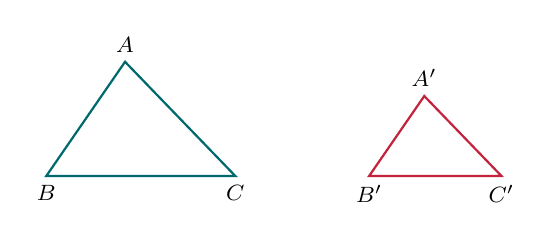
\begin{tikzpicture}[scale=1, font=\fontsize{9.5}{9.5}\selectfont]
  % Similar 1
  \coordinate (A) at (1.0, 1.45); \coordinate (B) at (0, 0); \coordinate (C) at (2.4, 0);
  \draw[thick, color=brandNavy] (A) -- (B) -- (C) -- cycle;
  \node[above] at (A) {\footnotesize $A$}; \node[below] at (B) {\footnotesize $B$}; \node[below] at (C) {\footnotesize $C$};

  % Similar 2 (smaller)
  \begin{scope}[xshift=4.1cm, scale=0.70]
    \coordinate (A1) at (1.0, 1.45); \coordinate (B1) at (0, 0); \coordinate (C1) at (2.4, 0);
    \draw[thick, color=brandCrimson] (A1) -- (B1) -- (C1) -- cycle;
    \node[above] at (A1) {\footnotesize $A'$}; \node[below] at (B1) {\footnotesize $B'$}; \node[below] at (C1) {\footnotesize $C'$};
  \end{scope}
\end{tikzpicture}\\[1pt]
{\small $\dfrac{AB}{A'B'} = \dfrac{BC}{B'C'} = \dfrac{CA}{C'A'} = k$}
\vspace{2pt}
\end{minipage} \tabularnewline \hline
\end{tabular}
\end{khcard}

\vspace{6pt}

\khsection{២}{ទំនាក់ទំនងមាត្រក្នុងត្រីកោណកែង}

\begin{khcard}[top=2pt, bottom=2pt, left=4pt, right=4pt]
\begin{minipage}[c]{0.66\textwidth}
\noindent\textbf{\color{brandNavy}\ding{70}\ ធាតុគ្រឹះនៃត្រីកោណកែង ៖} គេមានត្រីកោណ $ABC$ កែងត្រង់ $A$ និងមានកម្ពស់ $AH \perp BC$ ៖
\begin{itemize}[leftmargin=10pt, topsep=0pt, itemsep=0.2pt, parsep=0pt]
  \item $BC = a$ ៖ អ៊ីប៉ូតេនុស
  \item $AB = c$ \quad និង \quad $AC = b$ ៖ ជ្រុងនៃមុំកែង
  \item $AH = h$ ៖ កម្ពស់ត្រូវនឹងអ៊ីប៉ូតេនុស
  \item $BH = m$ (នៃ $c$) \quad និង \quad $CH = n$ (នៃ $b$) ៖ ចំណោលកែងលើអ៊ីប៉ូតេនុស
\end{itemize}
\end{minipage}\hfill
\begin{minipage}[c]{0.32\textwidth}
\centering
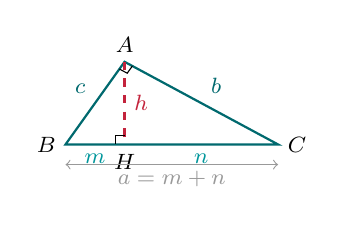
\begin{tikzpicture}[scale=0.75, font=\fontsize{8.5}{8.5}\selectfont]
  \coordinate (B) at (0,0); \coordinate (C) at (3.6,0);
  \coordinate (A) at (1.0,1.4); \coordinate (H) at (1.0,0);
  \draw[thick, color=brandNavy] (A) -- (B) -- (C) -- cycle;
  \draw[thick, dashed, color=brandCrimson] (A) -- (H);
  \node[above] at (A) {$A$}; \node[left] at (B) {$B$}; \node[right] at (C) {$C$};
  \node[below] at (H) {$H$};
  \node[above left] at ($(A)!0.5!(B)$) {\color{brandNavy} $c$};
  \node[above right] at ($(A)!0.5!(C)$) {\color{brandNavy} $b$};
  \node[right] at ($(A)!0.5!(H)$) {\color{brandCrimson} $h$};
  \node[below] at ($(B)!0.5!(H)$) {\color{brandTeal} $m$};
  \node[below] at ($(H)!0.5!(C)$) {\color{brandTeal} $n$};
  % Angle markers
  \draw[line width=0.4pt] (1.0,0.15) -- (0.85,0.15) -- (0.85,0);
  \draw[line width=0.4pt] ($(A)!0.15cm!(B)$) -- ++($(A)!0.15cm!(C)-(A)$) -- ($(A)!0.15cm!(C)$);
  % Double arrow for a
  \draw[<->, line width=0.4pt, color=gray!80] (0,-0.34) -- node[below=-1pt]{$a = m + n$} (3.6,-0.34);
\end{tikzpicture}
\end{minipage}
\end{khcard}

\vspace{1pt}

\begin{khcard}[top=2pt, bottom=2pt, left=4pt, right=4pt]
\noindent{\fontsize{8.5}{8.5}\selectfont\kml\color{brandCrimson}\textbf{\ding{45}\ តារាងសង្ខេបរូបមន្តទំនាក់ទំនងមាត្រទាំង ៥ ក្នុងត្រីកោណកែង}}
\par\vspace{1pt}
\centering
\renewcommand{\arraystretch}{1.0}
\fontsize{7.5}{8.5}\selectfont
\begin{tabular}{|c|l|l|c|}
\hline
\rowcolor{brandLightBlue}\textbf{ល.រ} & \textbf{ខ្លឹមសារធរណីមាត្រ} & \textbf{រូបមន្តតាមកំពូល} & \textbf{រូបមន្តតាមប្រវែង} \\ \hline
\textbf{១} & ការ៉េជ្រុងមុំកែង ស្មើ ផលគុណអ៊ីប៉ូតេនុស និងចំណោលរបស់វា & $AB^2 = BC \times BH, \ AC^2 = BC \times CH$ & \koreahl{$c^2 = a \cdot m, \ b^2 = a \cdot n$} \\ \hline
\textbf{២} & ការ៉េកម្ពស់ ស្មើ ផលគុណចំណោលកែងទាំងពីរ & $AH^2 = BH \times CH$ & \koreahl{$h^2 = m \cdot n$} \\ \hline
\textbf{៣} & ផលគុណជ្រុងមុំកែង ស្មើ ផលគុណអ៊ីប៉ូតេនុស និងកម្ពស់ & $AB \times AC = BC \times AH$ & \koreahl{$b \cdot c = a \cdot h$} \\ \hline
\textbf{៤} & ការ៉េអ៊ីប៉ូតេនុស ស្មើ ផលបូកការ៉េជ្រុងមុំកែង (ពីតាគ័រ) & $BC^2 = AB^2 + AC^2$ & \koreahl{$a^2 = b^2 + c^2$} \\ \hline
\textbf{៥} & ផលបូកច្រាសការ៉េជ្រុងមុំកែង ស្មើ ច្រាសការ៉េនៃកម្ពស់ & $\dfrac{1}{AH^2} = \dfrac{1}{AB^2} + \dfrac{1}{AC^2}$ & \koreahl{$\dfrac{1}{h^2} = \dfrac{1}{b^2} + \dfrac{1}{c^2}$} \\ \hline
\end{tabular}
\end{khcard}

\vspace{1pt}

\begin{khcard}[top=2pt, bottom=2pt, left=4pt, right=4pt]
\noindent{\fontsize{8}{8}\selectfont\kml\color{brandNavy}\textbf{\ding{70}\ សម្រាយបញ្ជាក់សង្ខេប ៖}}
\vspace{0.5pt}
\begin{itemize}[leftmargin=10pt, topsep=0pt, itemsep=0.1pt, parsep=0pt]
  \item \textbf{ទំនាក់ទំនងទី១ ៖} $\Delta ABC \sim \Delta HBA$ (ម.ម) $\implies \dfrac{AB}{BH} = \dfrac{BC}{AB} \implies AB^2 = BC \times BH$ (ដូចគ្នា $AC^2 = BC \times CH$)។
  \item \textbf{ទំនាក់ទំនងទី២ ៖} $\Delta ABH \sim \Delta CAH$ (ម.ម) $\implies \dfrac{AH}{CH} = \dfrac{BH}{AH} \implies AH^2 = BH \times CH$។
  \item \textbf{ទំនាក់ទំនងទី៣ ៖} $\Delta ABC \sim \Delta HBA$ (ម.ម) $\implies \dfrac{AC}{AH} = \dfrac{BC}{AB} \implies AB \times AC = BC \times AH$។
  \item \textbf{ទំនាក់ទំនងទី៤ ៖} តាម (១) បូកអង្គនិងអង្គ ៖ $AB^2 + AC^2 = BC(BH + CH) = BC^2$ (ទ្រឹស្ដីបទពីតាគ័រ)។
  \item \textbf{ទំនាក់ទំនងទី៥ ៖} តាម (៣) លើកជាការ៉េ ៖ $AB^2 \cdot AC^2 = BC^2 \cdot AH^2 = (AB^2 + AC^2)AH^2 \implies \dfrac{1}{AH^2} = \dfrac{1}{AB^2} + \dfrac{1}{AC^2}$។
\end{itemize}
\end{khcard}

\vspace{1pt}

\begin{multicols}{2}

\exhead{1} គេឱ្យត្រីកោណ $ABC$ កែងត្រង់ $A$ ដែល $AB=3\,\text{cm}$ និង $AC=4\,\text{cm}$ ។ ចូរគណនាប្រវែង $BC, AH, HB$ និង $HC$ ៖
\begin{center}\vspace{-6pt}
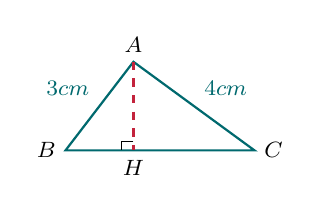
\begin{tikzpicture}[scale=0.75, font=\fontsize{8.5}{8.5}\selectfont]
  \coordinate (B) at (0,0); \coordinate (C) at (3.2,0);
  \coordinate (A) at (1.15,1.5); \coordinate (H) at (1.15,0);
  \draw[thick, color=brandNavy] (A) -- node[above left]{$3\text{cm}$} (B) -- (C) -- node[above right]{$4\text{cm}$} cycle;
  \draw[thick, dashed, color=brandCrimson] (A) -- (H);
  \node[above] at (A) {$A$}; \node[left] at (B) {$B$}; \node[right] at (C) {$C$}; \node[below] at (H) {$H$};
  \draw[line width=0.4pt] (1.15,0.15) -- (0.95,0.15) -- (0.95,0);
\end{tikzpicture}
\vspace{-6pt}\end{center}

\vspace{0.5pt}

\exhead{2} គេមានត្រីកោណ $ABC$ កែងត្រង់ $A$ ដែល $AH=8\,\text{cm}, BC=15\,\text{cm}$ និង $AC=12\,\text{cm}$ ។ ចូររកប្រវែងជ្រុង $AB, HB$ និង $HC$ ៖
\begin{center}\vspace{-6pt}
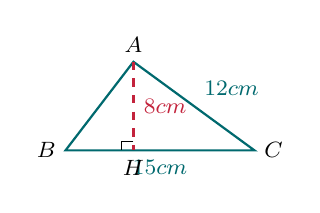
\begin{tikzpicture}[scale=0.75, font=\fontsize{8.5}{8.5}\selectfont]
  \coordinate (B) at (0,0); \coordinate (C) at (3.2,0);
  \coordinate (A) at (1.15,1.5); \coordinate (H) at (1.15,0);
  \draw[thick, color=brandNavy] (A) -- (B) -- node[below]{$15\text{cm}$} (C) -- node[above right]{$12\text{cm}$} cycle;
  \draw[thick, dashed, color=brandCrimson] (A) -- node[right]{$8\text{cm}$} (H);
  \node[above] at (A) {$A$}; \node[left] at (B) {$B$}; \node[right] at (C) {$C$}; \node[below] at (H) {$H$};
  \draw[line width=0.4pt] (1.15,0.15) -- (0.95,0.15) -- (0.95,0);
\end{tikzpicture}
\vspace{-6pt}\end{center}

\vspace{0.5pt}

\exhead{3} គេឱ្យត្រីកោណ $ABC$ កែងត្រង់ $A$ និងមានកម្ពស់ $AH$។ បើគេស្គាល់ $BH = 4\,\text{cm}$ និង $CH = 9\,\text{cm}$ ៖
\begin{center}\vspace{-6pt}
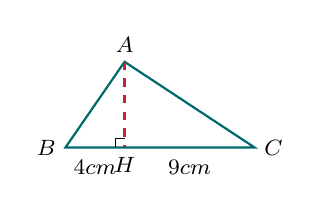
\begin{tikzpicture}[scale=0.75, font=\fontsize{8.5}{8.5}\selectfont]
  \coordinate (B) at (0,0);
  \coordinate (C) at (3.2,0);
  \coordinate (A) at (1.0, 1.45);
  \coordinate (H) at (1.0, 0);

  \draw[thick, color=brandNavy] (A) -- (B) -- (C) -- cycle;
  \draw[thick, dashed, color=brandCrimson] (A) -- (H);

  \node[above] at (A) {$A$};
  \node[left] at (B) {$B$};
  \node[right] at (C) {$C$};
  \node[below] at (H) {$H$};

  \node[below=1pt] at ($(B)!0.5!(H)$) {\fontsize{8}{8}\selectfont $4\text{cm}$};
  \node[below=1pt] at ($(H)!0.5!(C)$) {\fontsize{8}{8}\selectfont $9\text{cm}$};
  \draw[line width=0.4pt] (1.0,0.15) -- (0.85,0.15) -- (0.85,0);
\end{tikzpicture}
\vspace{-6pt}\end{center}
\begin{enumerate}[label=\alph*., topsep=0pt, itemsep=0.2pt, parsep=0pt, leftmargin=12pt]
  \item ចូរគណនាប្រវែងកម្ពស់ $AH$
  \item គណនាប្រវែងជ្រុង $AB, AC$ និងអ៊ីប៉ូតេនុស $BC$
\end{enumerate}

\columnbreak

\exhead{4} ក្នុងរូបខាងស្តាំនេះ អង្កត់ធ្នូ $CD$ និង $AB$ កាត់គ្នាត្រង់ $I$ ដែល $AI = 15\,\text{cm}, IC = 12\,\text{cm}, ID = 4\,\text{cm}, IB = 5\,\text{cm}, BD = 3\,\text{cm}$ ៖
\begin{center}\vspace{-6pt}
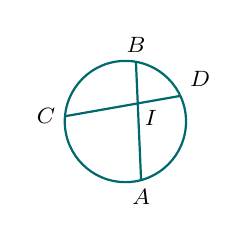
\begin{tikzpicture}[scale=0.7, font=\fontsize{8.5}{8.5}\selectfont]
  \coordinate (O) at (0,0);
  \draw[thick, color=brandNavy] (O) circle (1.1cm);
  
  \coordinate (A) at (-75:1.1cm);
  \coordinate (B) at (80:1.1cm);
  \coordinate (C) at (175:1.1cm);
  \coordinate (D) at (25:1.1cm);
  \coordinate (I) at (intersection of A--B and C--D);
  
  \draw[thick, color=brandNavy] (A) -- (B);
  \draw[thick, color=brandNavy] (C) -- (D);
  
  \node[below] at (A) {$A$};
  \node[above] at (B) {$B$};
  \node[left] at (C) {$C$};
  \node[above right] at (D) {$D$};
  \node[below right=-1pt] at (I) {$I$};
\end{tikzpicture}
\vspace{-6pt}\end{center}
\begin{enumerate}[label=\alph*., topsep=0pt, itemsep=0.2pt, parsep=0pt, leftmargin=12pt]
  \item ចូរប្រៀបធៀបត្រីកោណ $IAC$ និង $IBD$
  \item ចូរគណនារង្វាស់ $AC$
\end{enumerate}

\vspace{0.5pt}

\exhead{5} គេឱ្យត្រីកោណ $ABC$ ចារឹកក្នុងរង្វង់ ។ បន្ទាត់មួយស្របទៅនឹងបន្ទាត់ប៉ះត្រង់ $A$ កាត់អង្កត់ $AB$ និង $AC$ ត្រង់ចំណុច $M$ និង $N$ ៖
\begin{enumerate}[label=\alph*., topsep=0pt, itemsep=0.2pt, parsep=0pt, leftmargin=12pt]
  \item ចូរប្រដូចត្រីកោណ $ABC$ និង ត្រីកោណ $AMN$
  \item ចូរស្រាយបញ្ជាក់ថា $AB \cdot AM = AC \cdot AN$
\end{enumerate}

\vspace{0.5pt}

\exhead{6} ក្នុងរូបខាងស្តាំ ពីចំណុច $P$ គេគូសបន្ទាត់ប៉ះរង្វង់ត្រង់ $A$ ហើយគូសបន្ទាត់មួយទៀតកាត់រង្វង់ត្រង់ $C$ និង $D$ ៖
\begin{center}\vspace{-6pt}
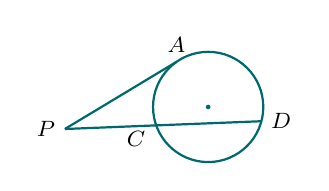
\begin{tikzpicture}[scale=0.7, font=\fontsize{8.5}{8.5}\selectfont]
  \coordinate (O) at (1.6, 0);
  \draw[thick, color=brandNavy] (O) circle (1.0cm);
  \fill[brandNavy] (O) circle (1.2pt);
  
  \coordinate (P) at (-1.0, -0.4);
  \coordinate (A) at ($(O)+(125:1.0cm)$);
  \draw[thick, color=brandNavy] (P) -- (A);
  
  \coordinate (C) at ($(O)+(195:1.0cm)$);
  \coordinate (D) at ($(O)+(-15:1.0cm)$);
  \draw[thick, color=brandNavy] (P) -- (D);
  
  \node[left] at (P) {$P$};
  \node[above] at (A) {$A$};
  \node[below left] at (C) {$C$};
  \node[right] at (D) {$D$};
\end{tikzpicture}
\vspace{-6pt}\end{center}
\begin{enumerate}[label=\alph*., topsep=0pt, itemsep=0.2pt, parsep=0pt, leftmargin=12pt]
  \item ចូរប្រៀបធៀបត្រីកោណ $PAC$ និង $PAD$
  \item ចូរទាញឱ្យឃើញថា $AP^2 = PC \times PD$
\end{enumerate}

\end{multicols}

\vspace{6pt}

% #########################################################################
% PAGE 5: ផ្នែកទី ៣ ៖ ទំនាក់ទំនងមាត្រក្នុងរង្វង់
% #########################################################################
\khsection{៣}{ទំនាក់ទំនងមាត្រក្នុងរង្វង់}

\khsubsection{៣.១}{ទ្រឹស្ដីបទតូឡេមី (Ptolemy's Theorem)}

\begin{khcard}[top=1pt, bottom=1pt, left=4pt, right=4pt]
\begin{minipage}[c]{0.64\textwidth}
\noindent\textbf{\color{brandNavy}\ding{70}\ ទ្រឹស្ដីបទតូឡេមី ៖}
បើចតុកោណ $ABCD$ មួយចារឹកក្នុងរង្វង់ នោះផលគុណនៃប្រវែងអង្កត់ទ្រូងទាំងពីរ ស្មើនឹងផលបូកនៃផលគុណប្រវែងជ្រុងឈមគ្នា ៖
\begin{center}
\koreahl{$AC \cdot BD = AB \cdot CD + AD \cdot BC$}
\end{center}
\vspace{0.5pt}
\noindent\textbf{\color{brandCrimson}\ding{45}\ សម្រាយបញ្ជាក់សង្ខេប ៖}
យក $E \in [BD]$ ដែល $\angle BAE = \angle CAD$ ៖
\begin{itemize}[leftmargin=10pt, topsep=0pt, itemsep=0.1pt, parsep=0pt]
  \item $\Delta ABE \sim \Delta ACD$ (ម.ម) $\implies \dfrac{AB}{BE} = \dfrac{AC}{CD} \implies AB \cdot CD = AC \cdot BE \quad (1)$
  \item $\Delta ABC \sim \Delta AED$ (ម.ម) $\implies \dfrac{AC}{BC} = \dfrac{AD}{ED} \implies AD \cdot BC = AC \cdot ED \quad (2)$
  \item បូក $(1)$ និង $(2)$ $\implies AB \cdot CD + AD \cdot BC = AC(BE + ED) = AC \cdot BD$ ។
\end{itemize}
\end{minipage}\hfill
\begin{minipage}[c]{0.34\textwidth}
\centering
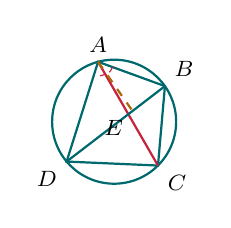
\begin{tikzpicture}[scale=0.75, font=\fontsize{8.5}{8.5}\selectfont]
  \coordinate (O) at (0,0);
  \draw[thick, color=brandNavy] (O) circle (1.05);
  \coordinate (A) at (105:1.05);
  \coordinate (B) at (35:1.05);
  \coordinate (C) at (-45:1.05);
  \coordinate (D) at (-140:1.05);
  
  \draw[thick, color=brandNavy] (A) -- (B) -- (C) -- (D) -- cycle;
  \draw[thick, color=brandCrimson] (A) -- (C);
  \draw[thick, color=brandNavy] (B) -- (D);
  
  \coordinate (E) at (intersection of A--{$(A)+(-55:2)$} and B--D);
  \draw[thick, dashed, color=brandGold!80!black] (A) -- (E);
  
  \node[above] at (A) {$A$};
  \node[above right] at (B) {$B$};
  \node[below right] at (C) {$C$};
  \node[below left] at (D) {$D$};
  \node[below left] at (E) {$E$};
  
  % Angle arcs
  \draw[line width=0.4pt, color=brandCrimson] ($(A)+(-82:0.24)$) arc (-82:-56:0.24);
  \draw[line width=0.4pt, color=brandCrimson] ($(A)+(-43:0.26)$) arc (-43:-18:0.26);
\end{tikzpicture}
\end{minipage}
\end{khcard}

\vspace{0.5pt}

\khsubsection{៣.២}{ស្វ័យគុណនៃមួយចំណុចចំពោះរង្វង់មួយ (Power of a Point)}

\begin{khcard}[top=1pt, bottom=1pt, left=4pt, right=4pt]
\begin{minipage}[c]{0.58\textwidth}
\noindent\textbf{\color{brandNavy}\ding{70}\ ទ្រឹស្ដីបទស្វ័យគុណនៃចំណុចមួយ ៖}
ចំពោះរង្វង់ $(O, R)$ និងចំណុច $P$ មួយ ៖
\begin{itemize}[leftmargin=10pt, topsep=0pt, itemsep=0.1pt, parsep=0pt]
  \item \textbf{ទ្រឹស្ដីបទ ១ ៖} បើ $P$ ជាចំណុចប្រសព្វ $AB$ និង $CD$ នោះ \koreahl{$PA \cdot PB = PC \cdot PD$}
  \item \textbf{ទ្រឹស្ដីបទ ២ ៖} បើ $PT$ ប៉ះរង្វង់ និង $PAB$ ជាបន្ទាត់កាត់ នោះ \koreahl{$PT^2 = PA \cdot PB$}
  \item \textbf{រូបមន្តស្វ័យគុណ $\mathcal{P}_{O}(P)$ ៖} $\mathcal{P}_{O}(P) = |OP^2 - R^2|$
    \begin{itemize}[leftmargin=8pt, topsep=0pt, itemsep=0pt]
      \item $P$ ខាងក្នុង ៖ $PA \cdot PB = R^2 - OP^2$
      \item $P$ ខាងក្រៅ ៖ $PA \cdot PB = OP^2 - R^2$
    \end{itemize}
  \item \textbf{វិបាក (Converse) ៖}
    \begin{itemize}[leftmargin=8pt, topsep=0pt, itemsep=0pt]
      \item $PA \cdot PB = PC \cdot PD \implies A, B, C, D$ លើរង្វង់តែមួយ
      \item $PA \cdot PB = PT^2 \implies PT$ ប៉ះរង្វង់ចារឹកក្រៅ $\Delta ABT$
    \end{itemize}
\end{itemize}
\end{minipage}\hfill
\begin{minipage}[c]{0.40\textwidth}
\centering
% Diagram 1: Interior intersecting chords
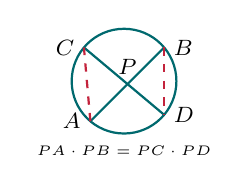
\begin{tikzpicture}[scale=0.7, font=\fontsize{8}{8}\selectfont]
  \draw[thick, color=brandNavy] (0,0) circle (0.95);
  \coordinate (A) at (-130:0.95); \coordinate (B) at (40:0.95);
  \coordinate (C) at (140:0.95); \coordinate (D) at (-40:0.95);
  \coordinate (P) at (intersection of A--B and C--D);
  \draw[thick, color=brandNavy] (A) -- (B); \draw[thick, color=brandNavy] (C) -- (D);
  \draw[thick, dashed, color=brandCrimson] (A) -- (C); \draw[thick, dashed, color=brandCrimson] (B) -- (D);
  \node[left] at (A) {$A$}; \node[right] at (B) {$B$};
  \node[left] at (C) {$C$}; \node[right] at (D) {$D$};
  \node[above] at (P) {$P$};
  \node[below] at (0,-1.0) {\fontsize{5.5}{5.5}\selectfont $PA \cdot PB = PC \cdot PD$};
\end{tikzpicture}\hspace{0.05cm}
% Diagram 2: Tangent & Secant
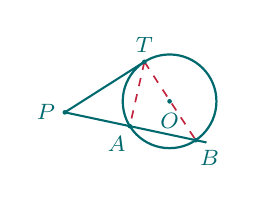
\begin{tikzpicture}[scale=0.7, font=\fontsize{8}{8}\selectfont]
  \coordinate (O) at (0,0);
  \draw[thick, color=brandNavy] (O) circle (0.85);
  \coordinate (P) at (-1.9,-0.2);
  \coordinate (T) at (122.5:0.85cm);
  \path[name path=secant] (P) -- ($(P)+(-12:3.3cm)$);
  \path[name path=circ] (O) circle (0.85cm);
  \path[name intersections={of=secant and circ, by={A,B}}];
  \draw[line width=0.75pt, brandNavy] (P) -- (T);
  \draw[line width=0.75pt, brandNavy] (P) -- ($(B)!-0.2cm!(P)$);
  \draw[line width=0.6pt, dashed, brandCrimson] (T) -- (A);
  \draw[line width=0.6pt, dashed, brandCrimson] (T) -- (B);
  \fill[brandNavy] (O) circle (1.2pt) node[below, yshift=-1pt]{$O$};
  \fill[brandNavy] (P) circle (1.2pt) node[left]{$P$};
  \fill[brandNavy] (T) circle (1.2pt) node[above]{$T$};
  \fill[brandNavy] (A) circle (1.2pt) node[below left, xshift=2pt]{$A$};
  \fill[brandNavy] (B) circle (1.2pt) node[below right, xshift=-2pt]{$B$};
\end{tikzpicture}
\end{minipage}
\end{khcard}

\vspace{-0.5cm}

\begin{multicols}{2}

\exhead{1} ក្នុងរូបខាងស្ដាំ ចំណុច $P$ នៅលើរង្វង់ចារឹកក្រៅ $\Delta ABC$។ យក $D, E, F$ ជាជើងចំណោលកែងនៃ $P$ មកលើជ្រុង $AB, BC, CA$ រៀងគ្នា ៖
\begin{center}\vspace{-6pt}
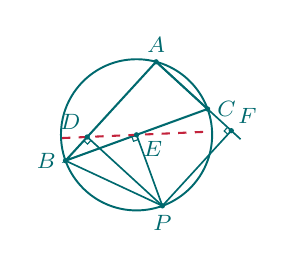
\begin{tikzpicture}[scale=0.8, font=\fontsize{8.5}{8.5}\selectfont]
  % Circumcircle
  \coordinate (O) at (0,0);
  \draw[line width=0.7pt, brandNavy] (O) circle (1.2cm);
  
  % Triangle ABC & Point P on circumcircle
  \coordinate (A) at (75:1.2cm);
  \coordinate (B) at (200:1.2cm);
  \coordinate (C) at (20:1.2cm);
  \coordinate (P) at (-70:1.2cm);
  
  % Projections D on AB, E on BC, F on line AC
  \coordinate (D) at ($(A)!(P)!(B)$);
  \coordinate (E) at ($(B)!(P)!(C)$);
  \coordinate (F) at ($(A)!(P)!(C)$);
  
  % Triangle ABC and line AC extended to F
  \draw[line width=0.75pt, brandNavy] (A) -- (B) -- (C) -- cycle;
  \draw[line width=0.6pt, brandNavy] (A) -- ($(F)!-0.2cm!(A)$);
  
  % Solid perpendicular segments PD, PE, PF
  \draw[line width=0.6pt, brandNavy] (P) -- (D);
  \draw[line width=0.6pt, brandNavy] (P) -- (E);
  \draw[line width=0.6pt, brandNavy] (P) -- (F);
  
  % Segment PB
  \draw[line width=0.6pt, brandNavy] (P) -- (B);
  
  % Right-angle mark at D
  \draw[line width=0.4pt, brandNavy] ($(D)!0.08cm!(B)$) -- ($($(D)!0.08cm!(B)$)+($(D)!0.08cm!(P)$)-(D)$) -- ($(D)!0.08cm!(P)$);
  
  % Right-angle mark at E
  \draw[line width=0.4pt, brandNavy] ($(E)!0.08cm!(B)$) -- ($($(E)!0.08cm!(B)$)+($(E)!0.08cm!(P)$)-(E)$) -- ($(E)!0.08cm!(P)$);
  
  % Right-angle mark at F
  \draw[line width=0.4pt, brandNavy] ($(F)!0.08cm!(C)$) -- ($($(F)!0.08cm!(C)$)+($(F)!0.08cm!(P)$)-(F)$) -- ($(F)!0.08cm!(P)$);
  
  % Dashed Simson Line passing through D, E, F
  \draw[line width=0.75pt, dashed, brandCrimson] ($(D)!-0.4cm!(F)$) -- ($(F)!0.4cm!(D)$);
  
  % Fill dots and labels
  \fill[brandNavy] (A) circle (1.2pt) node[above]{$A$};
  \fill[brandNavy] (B) circle (1.2pt) node[left]{$B$};
  \fill[brandNavy] (C) circle (1.2pt) node[right]{$C$};
  \fill[brandNavy] (P) circle (1.2pt) node[below]{$P$};
  
  \fill[brandNavy] (D) circle (1.2pt) node[above left=-1pt]{$D$};
  \fill[brandNavy] (E) circle (1.2pt) node[below right=-1pt]{$E$};
  \fill[brandNavy] (F) circle (1.2pt) node[above right=-1pt]{$F$};
\end{tikzpicture}
\vspace{-4pt}\end{center}
\begin{enumerate}[label=\alph*., topsep=0.5pt, itemsep=0.5pt, parsep=0pt, leftmargin=12pt]
  \item បង្ហាញថា $\angle PBD = \angle PEF$
  \item បង្ហាញថា បីចំណុច $D, E, F$ ស្ថិតនៅលើបន្ទាត់តែមួយ 
\end{enumerate}



\exhead{2} បកស្រាយបញ្ជាក់ទ្រឹស្ដីបទ ២ ៖ បើពីចំណុច $P$ ក្រៅរង្វង់ $O$ គេគូសបន្ទាត់មួយកាត់តាម $A$ និង $B$ លើរង្វង់ និងបន្ទាត់មួយទៀតប៉ះនឹងរង្វង់ $O$ ត្រង់ $T$ នោះគេបាន $PT^2 = PA \cdot PB$ ៖
\begin{center}\vspace{-6pt}
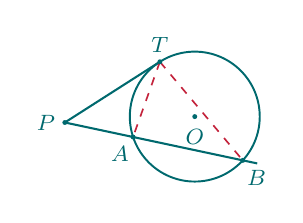
\begin{tikzpicture}[scale=0.75, font=\fontsize{8.5}{8.5}\selectfont]
  % Circle O
  \coordinate (O) at (0,0);
  \draw[line width=0.7pt, brandNavy] (O) circle (1.1cm);
  
  % Exterior point P
  \coordinate (P) at (-2.2, -0.1);
  \coordinate (T) at (122.5:1.1cm);
  
  \path[name path=secant] (P) -- ($(P)+(-12:3.6cm)$);
  \path[name path=circ] (O) circle (1.1cm);
  \path[name intersections={of=secant and circ, by={A,B}}];
  
  \draw[line width=0.75pt, brandNavy] (P) -- (T);
  \draw[line width=0.75pt, brandNavy] (P) -- ($(B)!-0.25cm!(P)$);
  
  \draw[line width=0.6pt, dashed, brandCrimson] (T) -- (A);
  \draw[line width=0.6pt, dashed, brandCrimson] (T) -- (B);
  
  \fill[brandNavy] (O) circle (1.2pt) node[below, yshift=-1pt]{$O$};
  \fill[brandNavy] (P) circle (1.2pt) node[left]{$P$};
  \fill[brandNavy] (T) circle (1.2pt) node[above]{$T$};
  \fill[brandNavy] (A) circle (1.2pt) node[below left, xshift=2pt]{$A$};
  \fill[brandNavy] (B) circle (1.2pt) node[below right, xshift=-2pt]{$B$};
\end{tikzpicture}
\vspace{-6pt}\end{center}



\exhead{3} គេមានចំណុច $P$ មួយនៅខាងក្រៅរង្វង់ $O$ កាំ $r$។ ដូចបង្ហាញក្នុងរូប បន្ទាត់កាត់តាម $P$ កាត់រង្វង់ត្រង់ $A, B$ និងបន្ទាត់ $OP$ កាត់រង្វង់ត្រង់ $C, D$ ៖
\begin{center}\vspace{-6pt}
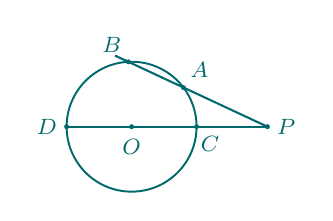
\begin{tikzpicture}[scale=0.75, font=\fontsize{8.5}{8.5}\selectfont]
  % Circle O with radius r = 1.1cm
  \coordinate (O) at (0,0);
  \draw[line width=0.7pt, brandNavy] (O) circle (1.1cm);
  
  % Exterior point P to the right
  \coordinate (P) at (2.3,0);
  
  % Center line OP cutting circle at C (near) and D (far)
  \coordinate (C) at (1.1,0);
  \coordinate (D) at (-1.1,0);
  \draw[line width=0.75pt, brandNavy] (D) -- (P);
  
  % Secant line PAB passing through A (near) and B (far)
  \path[name path=secant] (P) -- ($(P)+(155:3.8cm)$);
  \path[name path=circ] (O) circle (1.1cm);
  \path[name intersections={of=secant and circ, by={A,B}}];
  
  \draw[line width=0.75pt, brandNavy] (P) -- ($(B)!-0.25cm!(P)$);
  
  % Fill dots for points
  \fill[brandNavy] (O) circle (1.2pt) node[below, yshift=-1pt]{$O$};
  \fill[brandNavy] (P) circle (1.2pt) node[right]{$P$};
  \fill[brandNavy] (C) circle (1.2pt) node[below right, xshift=-2pt]{$C$};
  \fill[brandNavy] (D) circle (1.2pt) node[left]{$D$};
  \fill[brandNavy] (A) circle (1.2pt) node[above right, xshift=-1pt]{$A$};
  \fill[brandNavy] (B) circle (1.2pt) node[above left, xshift=1pt]{$B$};
\end{tikzpicture}
\vspace{-6pt}\end{center}
ចូរបង្ហាញថា $PA \cdot PB = OP^2 - r^2$។

\columnbreak

\exhead{4} ពីចំណុច $P$ ក្រៅរង្វង់ផ្ចិត $O$ គេគូសបន្ទាត់ $PA, PB$ ឱ្យប៉ះនឹងរង្វង់ ហើយយក $C$ ជាចំណុចប្រសព្វរវាង $AB$ និង $PO$។ បើអង្កត់ធ្នូ $DE$ ប្រសព្វ $PO$ ត្រង់ចំណុច $C$ ៖
\begin{center}\vspace{-6pt}
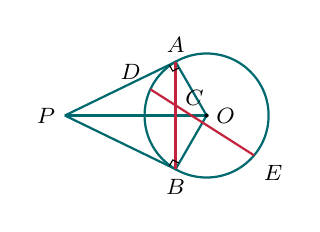
\begin{tikzpicture}[scale=0.75, font=\fontsize{8.5}{8.5}\selectfont]
  \coordinate (O) at (1.0,0);
  \draw[thick, color=brandNavy] (O) circle (1.05);
  \coordinate (P) at (-1.4,0);
  \coordinate (A) at ($(O)+(120:1.05)$);
  \coordinate (B) at ($(O)+(-120:1.05)$);
  \coordinate (C) at (intersection of A--B and P--O);
  
  \coordinate (D) at ($(O)+(155:1.05)$);
  \coordinate (E) at ($(O)+(-40:1.05)$);
  
  \draw[thick, color=brandNavy] (P) -- (A) -- (O);
  \draw[thick, color=brandNavy] (P) -- (B) -- (O);
  \draw[thick, color=brandNavy] (P) -- (O);
  \draw[thick, color=brandCrimson] (A) -- (B);
  \draw[thick, color=brandCrimson] (D) -- (E);
  
  \fill (O) circle (1pt) node[right]{$O$};
  \node[left] at (P) {$P$};
  \node[above] at (A) {$A$};
  \node[below] at (B) {$B$};
  \node[above right] at (C) {$C$};
  \node[above left] at (D) {$D$};
  \node[below right] at (E) {$E$};
  
  \draw[line width=0.4pt] ($(A)!0.12cm!(P)$) -- ++($(A)!0.12cm!(O)-(A)$) -- ($(A)!0.12cm!(O)$);
  \draw[line width=0.4pt] ($(B)!0.12cm!(P)$) -- ++($(B)!0.12cm!(O)-(B)$) -- ($(B)!0.12cm!(O)$);
\end{tikzpicture}
\vspace{-6pt}\end{center}
ចូរបង្ហាញថា បួនចំណុច $P, O, D, E$ ស្ថិតនៅលើរង្វង់តែមួយ។

\vspace{0.5pt}

\exhead{5} ស្រាយបញ្ជាក់វិបាក ៖
\begin{enumerate}[label=\alph*., topsep=1pt, itemsep=2pt, parsep=0pt, leftmargin=12pt]
  \item បើចំណុច $P$ នៅលើបន្លាយនៃអង្កត់ $AB$ និង $CD$ ដោយផ្ទៀងផ្ទាត់ $PA \cdot PB = PC \cdot PD$ នោះបួនចំណុច $A, B, C, D$ ស្ថិតនៅលើរង្វង់តែមួយ ៖
\begin{center}\vspace{-4pt}
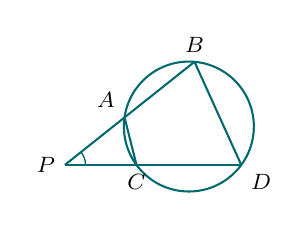
\begin{tikzpicture}[scale=0.75, font=\fontsize{8.5}{8.5}\selectfont]
  \coordinate (O) at (0,0);
  \draw[line width=0.75pt, brandNavy] (O) circle (1.1cm);
  
  \coordinate (P) at (-2.1, -0.65);
  \coordinate (C) at (-0.887, -0.65);
  \coordinate (D) at (0.887, -0.65);
  \coordinate (A) at (-1.089, 0.154);
  \coordinate (B) at (0.095, 1.096);
  
  % Secants PAB and PCD
  \draw[line width=0.75pt, brandNavy] (P) -- (B);
  \draw[line width=0.75pt, brandNavy] (P) -- (D);
  
  % Chords AC and BD
  \draw[line width=0.75pt, brandNavy] (A) -- (C);
  \draw[line width=0.75pt, brandNavy] (B) -- (D);
  
  % Angle arc at P
  \draw[line width=0.5pt, brandNavy] ($(P)+(0:0.35)$) arc (0:38.5:0.35);
  
  \node[left] at (P) {$P$};
  \node[above left] at (A) {$A$};
  \node[above] at (B) {$B$};
  \node[below] at (C) {$C$};
  \node[below right] at (D) {$D$};
\end{tikzpicture}
\vspace{-4pt}\end{center}

  \item បើបីចំណុច $A, B, T$ មិនស្ថិតនៅលើបន្ទាត់តែមួយ ហើយចំណុច $P$ នៅលើបន្លាយនៃអង្កត់ $AB$ ដោយផ្ទៀងផ្ទាត់ $PA \cdot PB = PT^2$ នោះបន្ទាត់ $PT$ ត្រូវប៉ះនឹងរង្វង់មួយដែលកាត់តាមបីចំណុច $A, B, T$ ៖
\begin{center}\vspace{-4pt}
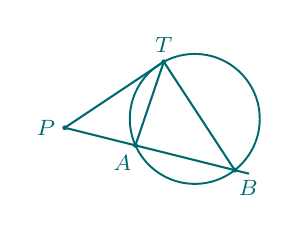
\begin{tikzpicture}[scale=0.75, font=\fontsize{8.5}{8.5}\selectfont]
  \coordinate (O) at (0,0);
  \draw[line width=0.7pt, brandNavy] (O) circle (1.1cm);
  
  \coordinate (P) at (-2.2, -0.15);
  \coordinate (T) at (118.5:1.1cm);
  
  \path[name path=secant] (P) -- ($(P)+(-14:3.6cm)$);
  \path[name path=circ] (O) circle (1.1cm);
  \path[name intersections={of=secant and circ, by={A,B}}];
  
  \draw[line width=0.75pt, brandNavy] (P) -- ($(B)!-0.25cm!(P)$);
  \draw[line width=0.75pt, brandNavy] (P) -- (T);
  \draw[line width=0.75pt, brandNavy] (T) -- (A);
  \draw[line width=0.75pt, brandNavy] (T) -- (B);
  
  \fill[brandNavy] (P) circle (1.2pt) node[left]{$P$};
  \fill[brandNavy] (T) circle (1.2pt) node[above]{$T$};
  \fill[brandNavy] (A) circle (1.2pt) node[below left, xshift=2pt]{$A$};
  \fill[brandNavy] (B) circle (1.2pt) node[below right, xshift=-2pt]{$B$};
\end{tikzpicture}
\vspace{-4pt}\end{center}
\end{enumerate}
\end{multicols}
\newpage
\par\Needspace*{4.0cm}
\begin{center}\vspace*{-4pt}
\begin{tcolorbox}[enhanced, colback=white, colframe=brandNavy!80, arc=4pt, boxrule=1pt, left=6pt, right=6pt, top=3pt, bottom=3pt, width=\textwidth]
  \fontfamily{kmfont}\selectfont
  \raisebox{-1pt}{\tikz[baseline={(0,-0.1)}]{\node[circle, draw=brandNavy, fill=brandNavy!10, line width=1.1pt, inner sep=2pt, font=\bfseries\sffamily\small\color{brandNavy}]{?};}}
  \hspace{4pt}
  {\fontsize{13}{13}\selectfont\kml\bfseries\color{brandNavy} លំហាត់}
  \hspace{6pt}
  \tikz[baseline={(0,0.15)}]{
    \draw[line width=1.5pt, brandNavy] (0,2.5pt) -- (10.2,2.5pt);
    \draw[line width=0.6pt, brandNavy] (0,-1pt) -- (10.2,-1pt);
  }
\end{tcolorbox}
\end{center}
\vspace{-4pt}

\begin{multicols}{2}

\exhead{1} គូត្រីកោណខាងក្រោមជាត្រីកោណដូចគ្នា ៖ សរសេរឈ្មោះនិងជ្រុងត្រូវគ្នា ៖
\begin{center}\vspace{-4pt}
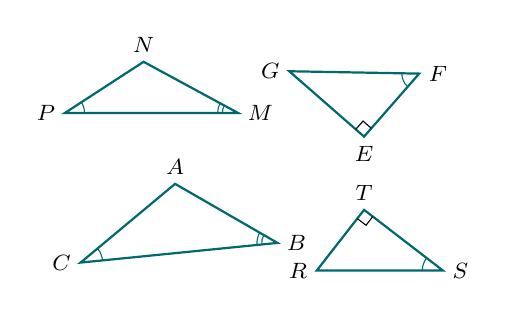
\begin{tikzpicture}[scale=1, font=\fontsize{8}{8}\selectfont]
  % Row 1: Left: Triangle PNM
  \coordinate (P) at (0,2.0);
  \coordinate (M) at (2.2,2.0);
  \coordinate (N) at (1.0,2.65);
  \draw[thick, brandNavy] (P) -- (N) -- (M) -- cycle;
  \node[left] at (P) {$P$}; \node[above] at (N) {$N$}; \node[right] at (M) {$M$};
  \draw[brandNavy, line width=0.4pt] ($(P)+(0:0.25)$) arc (0:34:0.25);
  \draw[brandNavy, line width=0.4pt] ($(M)+(180:0.2)$) arc (180:150:0.2);
  \draw[brandNavy, line width=0.4pt] ($(M)+(180:0.26)$) arc (180:150:0.26);

  % Row 1: Right: Triangle GFE
  \begin{scope}[xshift=2.8cm]
    \coordinate (E) at (1.0,1.7);
    \coordinate (F) at (1.7,2.5);
    \coordinate (G) at (0.05,2.53);
    \draw[thick, brandNavy] (G) -- (F) -- (E) -- cycle;
    \node[left] at (G) {$G$}; \node[right] at (F) {$F$}; \node[below] at (E) {$E$};
    \draw[line width=0.4pt] ($(E)!0.14cm!(G)$) -- ++($(E)!0.14cm!(F)-(E)$) -- ($(E)!0.14cm!(F)$);
    \draw[brandNavy, line width=0.4pt] ($(F)+(-135:0.22)$) arc (-135:-180:0.22);
  \end{scope}

  % Row 2: Left: Triangle CAB
  \coordinate (C) at (0.2,0.1);
  \coordinate (A) at (1.4,1.1);
  \coordinate (B) at (2.7,0.35);
  \draw[thick, brandNavy] (C) -- (A) -- (B) -- cycle;
  \node[left] at (C) {$C$}; \node[above] at (A) {$A$}; \node[right] at (B) {$B$};
  \draw[brandNavy, line width=0.4pt] ($(C)+(6:0.28)$) arc (6:40:0.28);
  \draw[brandNavy, line width=0.4pt] ($(B)+(186:0.2)$) arc (186:150:0.2);
  \draw[brandNavy, line width=0.4pt] ($(B)+(186:0.26)$) arc (186:150:0.26);

  % Row 2: Right: Triangle RTS
  \begin{scope}[xshift=3.0cm]
    \coordinate (R) at (0.2,0);
    \coordinate (S) at (1.8,0);
    \coordinate (T) at (0.8,0.77);
    \draw[thick, brandNavy] (R) -- (T) -- (S) -- cycle;
    \node[left] at (R) {$R$}; \node[above] at (T) {$T$}; \node[right] at (S) {$S$};
    \draw[line width=0.4pt] ($(T)!0.14cm!(R)$) -- ++($(T)!0.14cm!(S)-(T)$) -- ($(T)!0.14cm!(S)$);
    \draw[brandNavy, line width=0.4pt] ($(S)+(180:0.26)$) arc (180:142:0.26);
  \end{scope}
\end{tikzpicture}
\vspace{-4pt}\end{center}

\exhead{2} តើគូត្រីកោណនីមួយៗខាងក្រោមដូចគ្នាដែរឬទេ ? ហេតុអ្វី ?
\begin{center}\vspace{-4pt}
\begin{tikzpicture}[scale=1, font=\fontsize{7.5}{7.5}\selectfont]
  % Figure 1
  \begin{scope}[xshift=0cm]
    \coordinate (B) at (-1.4,1.2);
    \coordinate (A) at (0,1.2);
    \coordinate (C) at (0,0.3);
    \coordinate (D) at (0,0);
    \coordinate (E) at (2.0,0);
    \draw[thick, brandNavy] (B) -- (A) -- (D) -- (E);
    \draw[thick, brandNavy] (B) -- (C);
    \draw[thick, brandNavy] (A) -- (E);
    \node[left] at (B) {$B$}; \node[above] at (A) {$A$};
    \node[left] at (C) {$C$}; \node[below left] at (D) {$D$}; \node[right] at (E) {$E$};
    \draw[line width=0.4pt] (-0.14,1.2) -- (-0.14,1.06) -- (0,1.06);
    \draw[line width=0.4pt] (0,0.14) -- (0.14,0.14) -- (0.14,0);
    \node at (-0.9,1.02) {$57^\circ$};
    \node at (1.5,0.18) {$57^\circ$};
    \node[below] at (0.3,-0.15) {\scriptsize\bfseries រូបទី១};
  \end{scope}

  % Figure 2
  \begin{scope}[xshift=3.7cm]
    \coordinate (H) at (0.5,1.2);
    \coordinate (F) at (0,0);
    \coordinate (G) at (1.0,0);
    \draw[thick, brandNavy] (H) -- (F) -- (G) -- cycle;
    \node[above] at (H) {$H$}; \node[left] at (F) {$F$}; \node[right] at (G) {$G$};
    \node at (0.28,0.18) {$80^\circ$};
    \node at (0.8,0.18) {$70^\circ$};

    \begin{scope}[xshift=1.1cm]
      \coordinate (R) at (0,1.2);
      \coordinate (T) at (1.1,1.2);
      \coordinate (S) at (0.45,0.1);
      \draw[thick, brandNavy] (R) -- (T) -- (S) -- cycle;
      \node[above] at (R) {$R$}; \node[above] at (T) {$T$}; \node[below] at (S) {$S$};
      \node at (0.25,1.0) {$70^\circ$};
      \node at (0.5,0.38) {$40^\circ$};
    \end{scope}
    \node[below] at (1.05,-0.15) {\scriptsize\bfseries រូបទី២};
  \end{scope}
\end{tikzpicture}
\vspace{4pt}

\begin{tikzpicture}[scale=1, font=\fontsize{7.5}{7.5}\selectfont]
  % Figure 3: PL and MN horizontal
  \coordinate (P) at (0,1.2);
  \coordinate (L) at (2.0,1.2);
  \coordinate (M) at (-0.3,0);
  \coordinate (N_pt) at (1.8,0);
  
  \draw[thick, brandNavy] (P) -- (L);
  \draw[thick, brandNavy] (M) -- (N_pt);
  \draw[thick, brandNavy] (P) -- (N_pt);
  \draw[thick, brandNavy] (L) -- (M);
  
  \node[above left] at (P) {$P$}; \node[above right] at (L) {$L$};
  \node[below left] at (M) {$M$}; \node[below right] at (N_pt) {$N$};
  
  \node at (0.35,1.0) {$64^\circ$};
  \node at (0.9,0.85) {$102^\circ$};
  \node at (1.45,0.18) {$64^\circ$};
  \node[below right, yshift=2pt] at (0.95,0.58) {$N$};
  \node[below] at (0.85,-0.15) {\scriptsize\bfseries រូបទី៣};
\end{tikzpicture}
\vspace{-4pt}\end{center}

\exhead{3} ប្រៀបធៀប $\Delta ABC$ និង $\Delta A'B'C'$ , $\Delta PMN$ និង $\Delta P'M'N'$ រួចសរសេរផលធៀបដំណូច ៖
\begin{center}\vspace{-4pt}
\begin{tikzpicture}[scale=1, font=\fontsize{7.5}{7.5}\selectfont]
  % --- Figure 1: ABC and A'B'C' ---
  \begin{scope}[xshift=0cm]
    \coordinate (A) at (0.8,1.4);
    \coordinate (B) at (0,0.1);
    \coordinate (C) at (1.8,0.2);
    \draw[thick, brandNavy] (B) -- (A) -- (C) -- cycle;
    \node[above] at (A) {$A$}; \node[left] at (B) {$B$}; \node[right] at (C) {$C$};
    \draw[brandNavy, line width=0.4pt] ($(A)+(-115:0.22)$) arc (-115:-50:0.22);
    \draw[brandNavy, line width=0.4pt] ($(C)+(170:0.2)$) arc (170:125:0.2);
    \draw[brandNavy, line width=0.4pt] ($(C)+(170:0.26)$) arc (170:125:0.26);

    \begin{scope}[xshift=2.1cm]
      \coordinate (Bp) at (0,1.3);
      \coordinate (Cp) at (1.8,1.3);
      \coordinate (Ap) at (0.7,0.3);
      \draw[thick, brandNavy] (Bp) -- (Cp) -- (Ap) -- cycle;
      \node[left] at (Bp) {$B'$}; \node[right] at (Cp) {$C'$}; \node[below] at (Ap) {$A'$};
      \draw[brandNavy, line width=0.4pt] ($(Ap)+(60:0.22)$) arc (60:125:0.22);
      \draw[brandNavy, line width=0.4pt] ($(Cp)+(180:0.2)$) arc (180:215:0.2);
      \draw[brandNavy, line width=0.4pt] ($(Cp)+(180:0.26)$) arc (180:215:0.26);
    \end{scope}
    \node[below] at (1.9,-0.05) {\scriptsize\bfseries រូបទី១};
  \end{scope}
\end{tikzpicture}
\vspace{3pt}

\begin{tikzpicture}[scale=1, font=\fontsize{7.5}{7.5}\selectfont]
  % --- Figure 2: PMN and P'M'N' exactly matching book photo ---
  \begin{scope}[xshift=0cm]
    \coordinate (M) at (0,1.3);
    \coordinate (N) at (1.8,1.15);
    \coordinate (P) at (0.7,0.1);
    \draw[thick, brandNavy] (M) -- (N) -- (P) -- cycle;
    \node[left] at (M) {$M$}; \node[right] at (N) {$N$}; \node[below] at (P) {$P$};
    \draw[brandNavy, line width=0.4pt] ($(M)+(-60:0.22)$) arc (-60:0:0.22);
    \draw[brandNavy, line width=0.4pt] ($(P)+(120:0.2)$) arc (120:45:0.2);
    \draw[brandNavy, line width=0.4pt] ($(P)+(120:0.26)$) arc (120:45:0.26);

    \begin{scope}[xshift=2.0cm]
      \coordinate (Mp) at (0,0.55);
      \coordinate (Np) at (1.5,1.25);
      \coordinate (Pp) at (1.6,0.1);
      \draw[thick, brandNavy] (Mp) -- (Np) -- (Pp) -- cycle;
      \node[left] at (Mp) {$M'$}; \node[above] at (Np) {$N'$}; \node[right] at (Pp) {$P'$};
      \draw[brandNavy, line width=0.4pt] ($(Mp)+(-20:0.22)$) arc (-20:25:0.22);
      \draw[brandNavy, line width=0.4pt] ($(Pp)+(160:0.2)$) arc (160:95:0.2);
      \draw[brandNavy, line width=0.4pt] ($(Pp)+(160:0.26)$) arc (160:95:0.26);
    \end{scope}
    \node[below] at (1.75,-0.1) {\scriptsize\bfseries រូបទី២};
  \end{scope}
\end{tikzpicture}
\vspace{-4pt}\end{center}

\exhead{4} តើគូត្រីកោណនីមួយៗ ខាងក្រោមនេះជាត្រីកោណដូចគ្នាដែរឬទេ ? ហេតុអ្វី ?
\begin{center}\vspace{-4pt}
\begin{tikzpicture}[scale=1, font=\fontsize{7.5}{7.5}\selectfont]
  % Fig 1
  \begin{scope}[xshift=0cm]
    \coordinate (B) at (0,0);
    \coordinate (A) at (0.9,1.4);
    \coordinate (C) at (2.4,0.4);
    \coordinate (D) at (0.45,0.45);
    \coordinate (E) at (1.2,0.65);
    \draw[thick, brandNavy] (B) -- (A) node[midway, left]{14} -- (C) node[midway, above right]{16} -- cycle node[midway, below]{12};
    \draw[thick, brandNavy] (D) -- (E) node[midway, above]{8} -- ($(B)!0.5!(C)$) node[midway, below]{7} -- cycle node[midway, left]{6};
    \node[below] at (1.1,-0.25) {\scriptsize\bfseries រូបទី១};
  \end{scope}

  % Fig 2: horizontal bars
  \begin{scope}[xshift=3.3cm]
    \coordinate (TL) at (0,1.2); \coordinate (TR) at (1.6,1.2);
    \coordinate (BL) at (-0.6,0); \coordinate (BR) at (1.8,0);
    \draw[thick, brandNavy] (TL) -- (TR);
    \draw[thick, brandNavy] (BL) -- (BR);
    \draw[thick, brandNavy] (TL) -- (BR);
    \draw[thick, brandNavy] (TR) -- (BL);
    \node at (0.1,0.9) {16}; \node at (1.2,0.9) {10};
    \node at (-0.2,0.3) {32}; \node at (1.4,0.3) {20};
    \node[below] at (0.6,-0.25) {\scriptsize\bfseries រូបទី២};
  \end{scope}
\end{tikzpicture}
\vspace{3pt}

\begin{tikzpicture}[scale=1, font=\fontsize{7.5}{7.5}\selectfont]
  % Fig 3: vertical bars on left and right!
  \coordinate (TL) at (0,1.1); \coordinate (BL) at (0,-0.1);
  \coordinate (TR) at (2.0,1.1); \coordinate (BR) at (2.0,-0.1);
  \draw[thick, brandNavy] (TL) -- (BL);
  \draw[thick, brandNavy] (TR) -- (BR);
  \draw[thick, brandNavy] (TL) -- (BR);
  \draw[thick, brandNavy] (BL) -- (TR);
  \node at (0.7,0.95) {40}; \node at (1.5,0.95) {27};
  \node at (0.7,0.05) {36}; \node at (1.5,0.05) {30};
  \node[below] at (1.0,-0.25) {\scriptsize\bfseries រូបទី៣};
\end{tikzpicture}
\vspace{-4pt}\end{center}

\vfill\null\columnbreak

\exhead{5} គេឱ្យ $\Delta ABC \sim \Delta GEF$ រូបខាងក្រោម ៖ សរសេរបំពេញផលធៀបដំណូច ៖
\begin{center}\vspace{-2pt}
\begin{tikzpicture}[scale=1, font=\fontsize{7.5}{7.5}\selectfont]
  % Sub-part 1 (left): Triangles ABC and GEF stacked
  \begin{scope}[xshift=0cm]
    \coordinate (C) at (0,0.1); \coordinate (A) at (1.1,1.1); \coordinate (B) at (2.5,0.4);
    \draw[thick, brandNavy] (C) -- (A) -- (B) -- cycle;
    \node[left] at (C) {$C$}; \node[above] at (A) {$A$}; \node[right] at (B) {$B$};
    \draw[brandNavy, line width=0.4pt] ($(C)+(6:0.25)$) arc (6:40:0.25);
    \draw[brandNavy, line width=0.4pt] ($(B)+(187:0.2)$) arc (187:160:0.2);
    \draw[brandNavy, line width=0.4pt] ($(B)+(187:0.26)$) arc (187:160:0.26);

    \begin{scope}[yshift=-1.2cm]
      \coordinate (F) at (0.4,0); \coordinate (G) at (1.5,0.6); \coordinate (E) at (2.4,0.2);
      \draw[thick, brandNavy] (F) -- (G) -- (E) -- cycle;
      \node[left] at (F) {$F$}; \node[above] at (G) {$G$}; \node[right] at (E) {$E$};
      \draw[brandNavy, line width=0.4pt] ($(F)+(13:0.25)$) arc (13:30:0.25);
      \draw[brandNavy, line width=0.4pt] ($(E)+(187:0.2)$) arc (187:155:0.2);
      \draw[brandNavy, line width=0.4pt] ($(E)+(187:0.26)$) arc (187:155:0.26);
    \end{scope}
    \node at (1.3,-1.7) {\small $\dfrac{AB}{GE} = \dfrac{BC}{\boxed{\;\dots?\;}} = \dfrac{\boxed{\;\dots?\;}}{FG}$};
  \end{scope}

  % Sub-part 2 (right): Two right triangles facing each other
  \begin{scope}[xshift=3.7cm]
    \coordinate (B) at (0,0); \coordinate (C) at (0,1.1); \coordinate (A) at (1.3,0.25);
    \draw[thick, brandNavy] (C) -- (B) -- (A) -- cycle;
    \node[left] at (C) {$C$}; \node[left] at (B) {$B$}; \node[above] at (A) {$A$};
    \draw[line width=0.4pt] (0,0.12) -- (0.12,0.12) -- (0.12,0);
    \draw[brandNavy, line width=0.4pt] ($(A)+(145:0.22)$) arc (145:190:0.22);

    \begin{scope}[xshift=1.5cm]
      \coordinate (E) at (0,0.25); \coordinate (F) at (1.6,-0.1); \coordinate (G) at (1.5,1.2);
      \draw[thick, brandNavy] (E) -- (F) -- (G) -- cycle;
      \node[above] at (E) {$E$}; \node[below right] at (F) {$F$}; \node[above] at (G) {$G$};
      \draw[line width=0.4pt] ($(F)!0.12cm!(E)$) -- ++($(F)!0.12cm!(G)-(F)$) -- ($(F)!0.12cm!(G)$);
      \draw[brandNavy, line width=0.4pt] ($(E)+(-12:0.22)$) arc (-12:35:0.22);
      \draw[brandNavy, line width=0.4pt] ($(G)+(-90:0.2)$) arc (-90:-145:0.2);
      \draw[brandNavy, line width=0.4pt] ($(G)+(-90:0.26)$) arc (-90:-145:0.26);
    \end{scope}
    \node at (1.4,-1.7) {\small $\dfrac{AB}{EG} = \dfrac{\boxed{\;\dots?\;}}{EF} = \dfrac{BC}{\boxed{\;\dots?\;}}$};
  \end{scope}
\end{tikzpicture}
\vspace{-4pt}\end{center}

\exhead{6} ស្រាយបញ្ជាក់ថាត្រីកោណខាងក្រោមជាត្រីកោណដូចគ្នា រួចទាញវិបាក ៖
\begin{center}\vspace{-2pt}
\begin{tikzpicture}[scale=1, font=\fontsize{7.5}{7.5}\selectfont]
  % Left triangle ABC
  \coordinate (B) at (0,0);
  \coordinate (A) at (1.2,1.3);
  \coordinate (C) at (3.2,0.1);
  \draw[thick, brandNavy] (B) -- (A) node[midway, above left, xshift=2pt]{$348\,\text{m}$} -- (C) node[midway, above right, xshift=-2pt]{$290\,\text{m}$} -- cycle node[midway, below]{$400\,\text{m}$};
  \node[left] at (B) {$B$}; \node[above] at (A) {$A$}; \node[right] at (C) {$C$};
  \node at (0.35,0.18) {$58^\circ$}; \node at (1.2,1.05) {$77^\circ$};

  % Right triangle MNP
  \begin{scope}[xshift=3.7cm]
    \coordinate (M) at (0,0);
    \coordinate (N) at (0.9,0.95);
    \coordinate (P) at (2.0,0.05);
    \draw[thick, brandNavy] (M) -- (N) node[midway, above left, xshift=2pt]{$156.6\,\text{m}$} -- (P) node[midway, above right, xshift=-2pt]{$130.5\,\text{m}$} -- cycle node[midway, below]{$180\,\text{m}$};
    \node[left] at (M) {$M$}; \node[above] at (N) {$N$}; \node[right] at (P) {$P$};
    \node at (0.32,0.18) {$58^\circ$}; \node at (1.65,0.18) {$45^\circ$};
  \end{scope}
\end{tikzpicture}
\vspace{-4pt}\end{center}

\exhead{7} គេឱ្យចតុកោណព្នាយ $ABCD$ បន្លាយជ្រុងទ្រេត $AD$ និង $BC$ កាត់គ្នាត្រង់ $F$ ដោយស្គាល់ $FD : FA = 8 : 5$ និង $FB = 2.25\,\text{m}$ ៖ គណនាប្រវែង $BC$ ៖

\exhead{8} គេមានត្រីកោណដូចគ្នាពីរ ដែលមានបរិមាត្ររៀងគ្នា $35\,\text{dm}$ និង $56\,\text{dm}$ ៖ រកកម្ពស់មួយនៃត្រីកោណធំ បើកម្ពស់នៃត្រីកោណតូចស្មើនឹង $10\,\text{dm}$ ៖

\exhead{9} ក្នុងត្រីកោណ $ABC$ មាន $\angle BAC = 90^\circ$ ហើយ $RS \perp BC$ ៖ ស្រាយបញ្ជាក់ថា $\Delta ABC \sim \Delta SRC$ ៖
\begin{center}\vspace{-4pt}
\begin{tikzpicture}[scale=1, font=\fontsize{8}{8}\selectfont]
  \coordinate (A) at (0,1.6); \coordinate (B) at (0,0); \coordinate (C) at (3.5,1.6);
  \draw[thick, brandNavy] (A) -- (B) -- (C) -- cycle;
  \coordinate (R) at ($(A)!0.45!(C)$);
  \coordinate (S) at ($(B)!(R)!(C)$);
  \draw[thick, dashed, brandCrimson] (R) -- (S);
  \draw[line width=0.4pt] (0,1.42) -- (0.18,1.42) -- (0.18,1.6);
  \draw[line width=0.4pt] ($(S)!0.15cm!(R)$) -- ++($(S)!0.15cm!(B)-(S)$) -- ($(S)!0.15cm!(B)$);
  \node[left] at (A) {$A$}; \node[left] at (B) {$B$}; \node[above] at (C) {$C$};
  \node[above] at (R) {$R$}; \node[below right] at (S) {$S$};
\end{tikzpicture}
\vspace{-4pt}\end{center}

\exhead{10} ដោយចំណុច $C$ និង $D$ ដែលចែកអង្កត់ $MN$ ខាងក្នុងនិងខាងក្រៅតាមផលធៀប $\dfrac{a}{b}$ ៖
\begin{enumerate}[label=\alph*., topsep=1pt, itemsep=1pt, parsep=0pt, leftmargin=12pt]
  \item $MN = 11\,\text{dm}$, $\dfrac{a}{b} = \dfrac{3}{5}$
  \item $MN = 6\,\text{dm}$, $\dfrac{a}{b} = \dfrac{1}{3}$
\end{enumerate}
\begin{center}\vspace{-4pt}
\begin{tikzpicture}[scale=1, font=\fontsize{8}{8}\selectfont]
  \draw[thick, brandNavy] (0,0) -- (3.8,0.35);
  \draw[thick, dashed, brandNavy] (-1.2,-0.11) -- (0,0);
  \coordinate (D) at (-1.2,-0.11);
  \coordinate (M) at (0,0);
  \coordinate (C) at (2.0,0.18);
  \coordinate (N) at (3.8,0.35);
  \fill[brandNavy] (D) circle (1.2pt) node[above]{$D$};
  \fill[brandNavy] (M) circle (1.2pt) node[above]{$M$};
  \fill[brandNavy] (C) circle (1.2pt) node[above]{$C$};
  \fill[brandNavy] (N) circle (1.2pt) node[above]{$N$};
  \draw[line width=0.6pt] (2.0,0.08) -- (2.0,0.28);
\end{tikzpicture}
\vspace{-4pt}\end{center}

\vfill\null\newpage

\exhead{11} គេឱ្យត្រីកោណ $ABC$ ចារឹកក្នុងរង្វង់ដែល $AB = \alpha, AC = \beta, BC = \delta$ ៖ កន្លះបន្ទាត់ពុះ $\angle BAC$ កាត់ជ្រុង $BC$ ត្រង់ចំណុច $I$ និងកាត់ $BC$ ត្រង់ $J$ ៖
\begin{enumerate}[label=\alph*., topsep=1pt, itemsep=1pt, parsep=0pt, leftmargin=12pt]
  \item ស្រាយបញ្ជាក់ថា $\Delta ABI$ និង $\Delta AJC$ ជាត្រីកោណដូចគ្នា
  \item គណនាផលគុណ $AI \cdot AJ$
  \item បង្ហាញថា $\angle BAJ = \angle CBJ$
  \item ស្រាយបញ្ជាក់ថា $JB^2 = JA \cdot JI$
\end{enumerate}

\exhead{12} ដើម្បីវាស់ចម្ងាយពីចំណុច $A$ ទៅចំណុច $B$ ដែលមានឧបសគ្គមួយមិនអាចទៅដល់ គេជ្រើសរើសយកចំណុច $C$ មួយ រួចវាស់ប្រវែងអង្កត់ $AC$ ៖ បើ $D \in AC$ នោះវាស់អង្កត់ $CD$ តាមចំណុច $D$ គូសបន្ទាត់ $DE \parallel AB$ រួចវាស់អង្កត់ $DE$ ៖ ដោយធ្វើតាមរបៀបនេះ គេអាចគណនាអង្កត់ $AB$ បាន ៖ បើ $CA = 1800\,\text{m}, CD = 90\,\text{m}$ និង $DE = 150\,\text{m}$ ៖ គណនាចម្ងាយ $AB$ ៖
\begin{center}\vspace{-4pt}
\begin{tikzpicture}[scale=1, font=\fontsize{8}{8}\selectfont]
  \coordinate (A) at (-1.8,0.4);
  \coordinate (B) at (1.8,0.4);
  \coordinate (C) at (0.3,-1.4);
  \coordinate (D) at ($(C)!0.45!(A)$);
  \coordinate (E) at ($(C)!0.45!(B)$);
  
  % Mountain obstacle above AB matching textbook
  \fill[gray!18] (A) -- (-0.8,1.4) -- (0.4,2.0) -- (1.8,0.4) -- cycle;
  \fill[gray!35] (0.4,2.0) .. controls (0.8,1.6) and (1.1,1.2) .. (1.8,0.4) .. controls (1.2,0.8) and (0.6,0.6) .. (-0.1,0.85) .. controls (-0.7,0.65) and (-1.2,0.85) .. (A) .. controls (-0.7,1.2) .. (0.4,2.0) -- cycle;
  \draw[thick, brandNavy] (A) -- (-0.8,1.4) -- (0.4,2.0) -- (B);
  \draw[line width=0.5pt, brandNavy] (-1.5,0.65) .. controls (-0.7,0.45) and (0,0.75) .. (0.8,0.5) .. controls (1.2,0.65) .. (B);
  
  % Triangle below AB
  \draw[thick, brandNavy] (A) -- (B);
  \draw[thick, brandNavy] (A) -- (C) -- (B);
  \draw[thick, brandCrimson] (D) -- (E);
  
  \node[left] at (A) {$A$}; \node[right] at (B) {$B$}; \node[below] at (C) {$C$};
  \node[below left] at (D) {$D$}; \node[below right] at (E) {$E$};
\end{tikzpicture}
\vspace{-4pt}\end{center}

\exhead{13} គេឱ្យត្រីកោណ $ABC$ ចារឹកក្នុងរង្វង់ ៖ បន្ទាត់មួយស្របទៅនឹងបន្ទាត់ប៉ះត្រង់ $A$ កាត់អង្កត់ $AB$ និង $AC$ ត្រង់ចំណុច $M$ និង $N$ ៖
\begin{enumerate}[label=\alph*., topsep=1pt, itemsep=1pt, parsep=0pt, leftmargin=12pt]
  \item ប្រដូចត្រីកោណ $ABC$ និងត្រីកោណ $AMN$
  \item ស្រាយបញ្ជាក់ថា $AB \cdot AM = AC \cdot AN$
\end{enumerate}

\exhead{14} តាមចំណុចនៃកន្លះរង្វង់ គេគូសអង្កត់ $CD$ កែងទៅអង្កត់ផ្ចិត $AB$ ៖
\begin{enumerate}[label=\alph*., topsep=1pt, itemsep=1pt, parsep=0pt, leftmargin=12pt]
  \item បើ $AD = 4\,\text{dm}, DB = 9\,\text{dm}$ ៖ គណនា $CD$ ៖
  \item បើ $AB = 29\,\text{dm}, CD = 10\,\text{dm}$ ៖ គណនា $AD$ និង $DB$ ៖
\end{enumerate}

\exhead{15} ស្រាយបញ្ជាក់ថាក្នុងត្រីកោណមួយរង្វាស់កម្ពស់ច្រាសសមាមាត្រនឹងរង្វាស់ជ្រុងបាត $a h_a = b h_b = c h_c$ ៖
\par{\textcolor{gray!80}{\scriptsize\itshape ណែនាំ ៖ គូសកម្ពស់ពីររួចប្រដូចត្រីកោណកែងដែលមានកម្ពស់មួយជាជ្រុងកែង ៖}}

\exhead{16} តាមកំពូល $A$ នៃត្រីកោណសមបាត $ABC$ គេគូសបន្ទាត់មួយដែលកាត់ជ្រុង $BC$ ត្រង់ $D$ និងកាត់រង្វង់ចារឹកក្រៅត្រីកោណត្រង់ចំណុច $E$ ៖ ប្រៀបធៀបត្រីកោណ $ADB$ និងត្រីកោណ $AEB$ រួចស្រាយបញ្ជាក់ថា $AB^2 = AD \cdot AE$ ៖

\vfill\null\columnbreak

\exhead{17} ដើមឫស្សីមួយដើមមានកម្ពស់ $10\,\text{m}$ ត្រូវខ្យល់បាក់បត់ត្រង់ចំណុច $P$ មួយ ហើយចុងឫស្សីប៉ះដីត្រង់ចំណុចមួយដែលមានចម្ងាយ $3\,\text{m}$ ពីគល់ ៖ គណនាដើមឫស្សីពីគល់ទៅចំណុចបាក់ $P$ ៖

\exhead{18} $AB$ ជាជម្រៅទឹកដល់បាតស្មៅឈូក ហើយផ្នែកផុតពីទឹកមានប្រវែង $AE = 3\,\text{dm}$ ពេលនោះមានខ្យល់បក់ធ្វើឱ្យស្មៅឈូកទ្រេតប្រកាន់យកស្ថានភាព $BA'$ ដែល $EA' = 9\,\text{dm}$ ៖ រកជម្រៅទឹក $EB$ ៖
\begin{center}\vspace{-4pt}
\begin{tikzpicture}[scale=1, font=\fontsize{8}{8}\selectfont]
  % Pond bed
  \fill[gray!30] (-0.5,-0.3) .. controls (0.5,-0.1) and (1.5,-0.4) .. (3.2,-0.2) -- (3.2,-0.5) -- (-0.5,-0.5) -- cycle;
  \draw[thick, brandNavy] (-0.5,-0.3) .. controls (0.5,-0.1) and (1.5,-0.4) .. (3.2,-0.2);

  % Water surface
  \draw[line width=0.8pt, teal!70] (-0.5,1.0) -- (3.2,1.0);
  \fill[teal!10, opacity=0.5] (-0.5,-0.2) rectangle (3.2,1.0);

  % Points
  \coordinate (B) at (1.0,-0.2);
  \coordinate (E) at (1.0,1.0);
  \coordinate (A) at (1.0,1.6);
  \coordinate (Ap) at (2.6,1.0);

  % Upright stem
  \draw[line width=1.5pt, brandNavy] (B) -- (A);
  % Bent stem
  \draw[line width=1.5pt, brandNavy] (B) -- (Ap);
  % Dashed connecting line
  \draw[thick, dashed, brandCrimson] (A) -- (Ap);
  \draw[thick, brandNavy] (E) -- (Ap);

  % Right angle at E
  \draw[line width=0.4pt] (1.0,1.15) -- (1.15,1.15) -- (1.15,1.0);

  % Lotus bud at A
  \draw[fill=brandCrimson!20, draw=brandCrimson, thick] (A) .. controls (0.85,1.8) and (0.95,2.1) .. (1.0,2.2) .. controls (1.05,2.1) and (1.15,1.8) .. (A);
  % Floating bud at Ap
  \draw[fill=brandCrimson!20, draw=brandCrimson, thick] (Ap) .. controls (2.45,1.2) and (2.55,1.5) .. (2.6,1.6) .. controls (2.65,1.5) and (2.75,1.2) .. (Ap);

  \node[left] at (A) {$A$};
  \node[left] at (E) {$E$};
  \node[below] at (B) {$B$};
  \node[below] at (Ap) {$A'$};

  \node[left] at (1.0,1.3) {$3\,\text{dm}$};
  \node[above] at (1.8,1.0) {$9\,\text{dm}$};
\end{tikzpicture}
\vspace{-4pt}\end{center}

\exhead{19} តាង $b$ និង $c$ ជាជើងនៃជ្រុងទាំងពីរនៃមុំកែងរបស់ត្រីកោណកែងមួយ ៖ $h$ ជាជើងនៃរង្វាស់កម្ពស់ចំពោះអ៊ីប៉ូតែនុស ៖ គណនា $h$ ទៅតាមតម្លៃ $a$ និង $b$ ៖

\exhead{20} $ABCD$ ជាប្រលឡូក្រាមដូចរូបខាងស្តាំ ៖ $I$ ជាចំណុចកណ្ដាលនៃ $AD$ ដែល $IB \perp AD$ ៖
\begin{enumerate}[label=\alph*., topsep=1pt, itemsep=1pt, parsep=0pt, leftmargin=12pt]
  \item គណនា $IB$
  \item គណនាផ្ទៃក្រឡានៃប្រលឡូក្រាម
\end{enumerate}
\begin{center}\vspace{-4pt}
\begin{tikzpicture}[scale=1, font=\fontsize{8}{8}\selectfont]
  \coordinate (A) at (0,0);
  \coordinate (D) at (0.64,1.6);
  \coordinate (B) at (2.32,0);
  \coordinate (C) at (2.96,1.6);
  
  \draw[thick, brandNavy] (A) -- (B) -- (C) -- (D) -- cycle;
  \coordinate (I) at ($(A)!0.5!(D)$);
  
  \draw[thick, brandNavy] (I) -- (B);
  \draw[line width=0.4pt] ($(I)!0.14cm!(A)$) -- ++($(I)!0.14cm!(B)-(I)$) -- ($(I)!0.14cm!(B)$);
  
  % Tick marks on AI and ID
  \draw[line width=0.6pt] ($(A)!0.25!(I)+(110:0.07)$) -- ($(A)!0.25!(I)+(-70:0.07)$);
  \draw[line width=0.6pt] ($(A)!0.25!(I)+(110:0.07)+(30:0.03)$) -- ($(A)!0.25!(I)+(-70:0.07)+(30:0.03)$);
  \draw[line width=0.6pt] ($(I)!0.25!(D)+(110:0.07)$) -- ($(I)!0.25!(D)+(-70:0.07)$);
  \draw[line width=0.6pt] ($(I)!0.25!(D)+(110:0.07)+(30:0.03)$) -- ($(I)!0.25!(D)+(-70:0.07)+(30:0.03)$);

  \node[below left] at (A) {$A$};
  \node[below right] at (B) {$B$};
  \node[above right] at (C) {$C$};
  \node[above left] at (D) {$D$};
  \node[left] at (I) {$I$};
  
  \node[below] at (1.16,0) {\scriptsize $10\,\text{cm}$};
  \node[right] at (2.64,0.8) {\scriptsize $12\,\text{cm}$};
\end{tikzpicture}
\vspace{-4pt}\end{center}

\exhead{21} ក្នុងរូបខាងស្តាំនេះ $NMQ$ និង $PNQ$ ជាត្រីកោណកែង ៖
\begin{enumerate}[label=\alph*., topsep=1pt, itemsep=1pt, parsep=0pt, leftmargin=12pt]
  \item គណនារង្វាស់ $MQ$
  \item គណនារង្វាស់ $NP$
\end{enumerate}
\begin{center}\vspace{-4pt}
\begin{tikzpicture}[scale=1, font=\fontsize{8}{8}\selectfont]
  % Right triangle NMQ right at M: MN=1.65 (3cm), MQ=2.2 (4cm), NQ=2.75 (5cm)
  \coordinate (M) at (0,0);
  \coordinate (N) at (0,1.65);
  \coordinate (Q) at (2.2,0);
  
  % Right triangle PNQ right at N: QN vector is (-2.2, 1.65) = 2.75 * (-0.8, 0.6)
  % Perp vector is (0.6, 0.8). Length NP = 2.75 * 0.75 = 2.06
  \coordinate (P) at ($(N) + (2.06*0.6, 2.06*0.8)$);
  
  \draw[thick, brandNavy] (M) -- (Q) -- (P) -- (N) -- cycle;
  \draw[thick, brandNavy] (N) -- (Q);
  
  % Right angle at M
  \draw[line width=0.4pt] (0,0.18) -- (0.18,0.18) -- (0.18,0);
  % Right angle at N (between NQ and NP)
  \draw[line width=0.4pt] ($(N)!0.16cm!(P)$) -- ++($(N)!0.16cm!(Q)-(N)$) -- ($(N)!0.16cm!(Q)$);
  
  % Equal angle arcs at Q
  \draw[brandNavy, line width=0.4pt] ($(Q)+(180:0.42)$) arc (180:143.13:0.42);
  \draw[brandNavy, line width=0.4pt] ($(Q)+(143.13:0.46)$) arc (143.13:106.26:0.46);

  \node[left] at (M) {$M$};
  \node[left] at (N) {$N$};
  \node[above] at (P) {$P$};
  \node[right] at (Q) {$Q$};
  
  \node[left] at (0,0.85) {\scriptsize $3\,\text{cm}$};
  \node[above] at (1.1,0.8) {\scriptsize $5\,\text{cm}$};
\end{tikzpicture}
\vspace{-4pt}\end{center}

\exhead{22} ក្នុងរូបខាងស្តាំ អង្កត់ធ្នូ $CD$ និង $AB$ កាត់គ្នាត្រង់ $I$ ដែល $AI = 15\,\text{cm}$, $IC = 12\,\text{cm}$, $ID = 4\,\text{cm}$, $IB = 5\,\text{cm}$ ៖
\begin{enumerate}[label=\alph*., topsep=1pt, itemsep=1pt, parsep=0pt, leftmargin=12pt]
  \item ប្រៀបធៀបត្រីកោណ $IAC$ និង $IBD$
  \item គណនារង្វាស់ $AC$
\end{enumerate}
\begin{center}\vspace{-4pt}
\begin{tikzpicture}[scale=1, font=\fontsize{8}{8}\selectfont]
  \coordinate (O) at (0,0);
  \draw[line width=0.6pt, brandNavy] (O) circle (1.3cm);
  
  \coordinate (A) at (-75:1.3cm);
  \coordinate (B) at (80:1.3cm);
  \coordinate (C) at (175:1.3cm);
  \coordinate (D) at (10:1.3cm);
  
  \draw[thick, brandNavy] (A) -- (B);
  \draw[thick, brandNavy] (C) -- (D);
  \path [name path=AB] (A) -- (B);
  \path [name path=CD] (C) -- (D);
  \path [name intersections={of=AB and CD, by={I}}];
  
  \node[below] at (A) {$A$};
  \node[above] at (B) {$B$};
  \node[left] at (C) {$C$};
  \node[right] at (D) {$D$};
  \node[above left] at (I) {$I$};
\end{tikzpicture}
\vspace{-4pt}\end{center}

\vfill\null\newpage

\exhead{23} ក្នុងរូបខាងស្តាំពីចំណុច $P$ គេគូសបន្ទាត់ប៉ះរង្វង់ត្រង់ $A$ ហើយគូសបន្ទាត់មួយទៀតកាត់រង្វង់ត្រង់ $C$ និង $D$ ៖
\begin{enumerate}[label=\alph*., topsep=1pt, itemsep=1pt, parsep=0pt, leftmargin=12pt]
  \item ប្រៀបធៀបត្រីកោណ $PAC$ និង $PAD$
  \item ទាញឱ្យឃើញថា $AP^2 = PC \times PD$
\end{enumerate}
\begin{center}\vspace{-4pt}
\begin{tikzpicture}[scale=1, font=\fontsize{8}{8}\selectfont]
  \coordinate (O) at (1.8,0.7);
  \draw[line width=0.6pt, brandNavy] (O) circle (1.2cm);
  \fill[brandNavy] (O) circle (1.2pt);
  
  \coordinate (P) at (-1.2,0.1);
  % Exact tangent point from P to circle at (1.8, 0.7) with R=1.2
  \coordinate (A) at (1.12,1.69);
  \coordinate (C) at (0.61,0.32);
  \coordinate (D) at (2.99,0.61);
  
  \draw[thick, brandNavy] (P) -- (A);
  \draw[thick, brandNavy] (P) -- (D);
  
  \fill[brandNavy] (A) circle (1.2pt) node[above]{$A$};
  \fill[brandNavy] (C) circle (1.2pt) node[below left]{$C$};
  \fill[brandNavy] (D) circle (1.2pt) node[right]{$D$};
  \node[left] at (P) {$P$};
\end{tikzpicture}
\vspace{-4pt}\end{center}

\exhead{24} ក្នុងរូបខាងស្តាំ តើកោនទាំងពីរដូចគ្នាឬទេ ?
\begin{center}\vspace{-4pt}
\begin{tikzpicture}[scale=1, font=\fontsize{8}{8}\selectfont]
  % Small Cone
  \begin{scope}[xshift=0cm]
    \draw[thick, brandNavy] (-0.65,0) arc (180:360:0.65cm and 0.18cm);
    \draw[dashed, brandNavy] (0.65,0) arc (0:180:0.65cm and 0.18cm);
    \draw[thick, brandNavy] (-0.65,0) -- (0,1.7) -- (0.65,0);
    \draw[thick, brandNavy] (0,0) -- (0,1.7);
    
    % Height dimension on right
    \draw[<->, line width=0.4pt, brandNavy] (0.8,0) -- (0.8,1.7) node[midway, right]{$5\,\text{cm}$};
    % Diameter dimension below
    \draw[<->, line width=0.4pt, brandNavy] (-0.65,-0.3) -- (0.65,-0.3) node[midway, below]{$4\,\text{cm}$};
  \end{scope}

  % Large Cone
  \begin{scope}[xshift=2.5cm]
    \draw[thick, brandNavy] (-1.1,0) arc (180:360:1.1cm and 0.28cm);
    \draw[dashed, brandNavy] (1.1,0) arc (0:180:1.1cm and 0.28cm);
    \draw[thick, brandNavy] (-1.1,0) -- (0,2.5) -- (1.1,0);
    \draw[thick, brandNavy] (0,0) -- (0,2.5);
    
    % Height dimension on right
    \draw[<->, line width=0.4pt, brandNavy] (1.3,0) -- (1.3,2.5) node[midway, right]{$10\,\text{cm}$};
    % Diameter dimension below
    \draw[<->, line width=0.4pt, brandNavy] (-1.1,-0.4) -- (1.1,-0.4) node[midway, below]{$8\,\text{cm}$};
  \end{scope}
\end{tikzpicture}
\vspace{-4pt}\end{center}

\exhead{25} រូបខាងស្តាំជាកោនពីរដូចគ្នា ៖
\begin{enumerate}[label=\alph*., topsep=1pt, itemsep=1pt, parsep=0pt, leftmargin=12pt]
  \item បង្ហាញថាបើកោនពីរដូចគ្នានោះ $\dfrac{v}{V} = \left(\dfrac{h}{H}\right)^3 = \left(\dfrac{r}{R}\right)^3$ ដែល $v$ និង $V$ ជាមាឌ
  \item បើកោនតូចមានមាឌ $v = 6.28\,\text{cm}^3$ ហើយ $h = 2\,\text{cm}$, $H = 4\,\text{cm}$ ៖ គណនាមាឌ $V$ នៃកោនធំ ៖
\end{enumerate}
\begin{center}\vspace{-4pt}
\begin{tikzpicture}[scale=1, font=\fontsize{8}{8}\selectfont]
  % Small Cone
  \begin{scope}[xshift=0cm]
    \draw[thick, brandNavy] (-0.6,0) arc (180:360:0.6cm and 0.16cm);
    \draw[dashed, brandNavy] (0.6,0) arc (0:180:0.6cm and 0.16cm);
    \draw[thick, brandNavy] (-0.6,0) -- (0,1.5) -- (0.6,0);
    \draw[thick, brandNavy] (0,0) -- (0,1.5);
    
    % Guidelines & height
    \draw[dashed, gray] (0,1.5) -- (0.8,1.5);
    \draw[dashed, gray] (0.6,0) -- (0.8,0);
    \draw[<->, line width=0.4pt, brandNavy] (0.8,0) -- (0.8,1.5) node[midway, right]{$h$};
    
    % Radius below
    \draw[dashed, gray] (0,0) -- (0,-0.3);
    \draw[dashed, gray] (0.6,0) -- (0.6,-0.3);
    \draw[<->, line width=0.4pt, brandNavy] (0,-0.25) -- (0.6,-0.25) node[midway, below]{$r$};
  \end{scope}

  % Large Cone
  \begin{scope}[xshift=2.4cm]
    \draw[thick, brandNavy] (-1.1,0) arc (180:360:1.1cm and 0.26cm);
    \draw[dashed, brandNavy] (1.1,0) arc (0:180:1.1cm and 0.26cm);
    \draw[thick, brandNavy] (-1.1,0) -- (0,2.5) -- (1.1,0);
    \draw[thick, brandNavy] (0,0) -- (0,2.5);
    
    % Guidelines & height
    \draw[dashed, gray] (0,2.5) -- (1.3,2.5);
    \draw[dashed, gray] (1.1,0) -- (1.3,0);
    \draw[<->, line width=0.4pt, brandNavy] (1.3,0) -- (1.3,2.5) node[midway, right]{$H$};
    
    % Radius below
    \draw[dashed, gray] (0,0) -- (0,-0.35);
    \draw[dashed, gray] (1.1,0) -- (1.1,-0.35);
    \draw[<->, line width=0.4pt, brandNavy] (0,-0.3) -- (1.1,-0.3) node[midway, below]{$R$};
  \end{scope}
\end{tikzpicture}
\vspace{-4pt}\end{center}

\vfill\null\columnbreak

\exhead{26} គេមាន $\Delta ABC$ និងចំណុច $P$ នៅលើបន្លាយនៃ $AB$ ដូចរូបខាងស្តាំ ៖ គេដឹងថា $AB = BP = 3, PC = 3\sqrt{2}$ ៖
\begin{enumerate}[label=\alph*., topsep=1pt, itemsep=1pt, parsep=0pt, leftmargin=12pt]
  \item បង្ហាញថា $PC$ ប៉ះនឹងរង្វង់ចារឹកក្រៅ $\Delta ABC$
  \item បើ $BC = \sqrt{3}$ ៖ កំណត់ប្រវែងជ្រុង $AC$ ៖
  \par បង្ហាញថាជ្រុង $AB$ ជាអង្កត់ផ្ចិតនៃរង្វង់ចារឹកក្រៅ $\Delta ABC$ ៖
\end{enumerate}
\begin{center}\vspace{-4pt}
\begin{tikzpicture}[scale=1, font=\fontsize{8}{8}\selectfont]
  \coordinate (O) at (0,0);
  \draw[line width=0.6pt, brandNavy] (O) circle (1.2cm);
  
  \coordinate (C) at (0,1.2);
  \coordinate (P) at (3.39,1.2);
  
  % Exact diameter AB passing through center (0,0) collinear with P(3.39, 1.2)
  \coordinate (A) at (-1.13,-0.40);
  \coordinate (B) at (1.13,0.40);
  
  \draw[thick, brandNavy] (C) -- (P);
  \draw[thick, brandNavy] (A) -- (B);
  \draw[thick, dashed, brandNavy] (B) -- (P);
  \draw[thick, brandNavy] (A) -- (C) -- (B);
  
  \fill[brandNavy] (A) circle (1.2pt) node[below left]{$A$};
  \fill[brandNavy] (B) circle (1.2pt) node[above left, xshift=1pt]{$B$};
  \fill[brandNavy] (C) circle (1.2pt) node[above left]{$C$};
  \fill[brandNavy] (P) circle (1.2pt) node[right]{$P$};
  
  % Dimension line for CP
  \draw[<->, dashed, brandNavy, line width=0.4pt] ($(C)+(0,0.18)$) -- ($(P)+(0,0.18)$) node[midway, above]{$3\sqrt{2}$};
  % Numbers 3 for AB and BP
  \node[below right] at ($(A)!0.5!(B)$) {\scriptsize $3$};
  \node[below right] at ($(B)!0.5!(P)$) {\scriptsize $3$};
\end{tikzpicture}
\vspace{-4pt}\end{center}

\exhead{27} គេដៅចំណុច $P$ នៅលើអង្កត់ធ្នូរួមរវាងពីររង្វង់ដែលប្រសព្វគ្នា ហើយពីចំណុច $P$ នេះ គេគូសអង្កត់ធ្នូ $AB, CD$ ដូចរូប ៖ បង្ហាញថា $4$ ចំណុច $A, B, C, D$ ស្ថិតនៅលើរង្វង់តែមួយ ៖
\begin{center}\vspace{-4pt}
\begin{tikzpicture}[scale=1, font=\fontsize{8}{8}\selectfont]
  \coordinate (O1) at (0,0);
  \coordinate (O2) at (1.2,0);
  
  \draw[line width=0.6pt, brandNavy] (O1) circle (1.2cm);
  \draw[line width=0.6pt, brandNavy] (O2) circle (0.95cm);
  
  % Common chord (radical axis)
  \draw[thick, brandNavy] (0.824, 0.872) -- (0.824, -0.872);
  \coordinate (P) at (0.824, 0.080);
  
  % Chord AB through P (A on C1, B on C2)
  \coordinate (A) at (-0.983, -0.688);
  \coordinate (B) at (1.964, 0.565);
  \draw[thick, brandNavy] (A) -- (B);
  
  % Chord CD through P (C on C1, D on C2)
  \coordinate (C) at (-0.688, 0.983);
  \coordinate (D) at (1.945, -0.589);
  \draw[thick, brandNavy] (C) -- (D);
  
  \fill[brandNavy] (P) circle (1.2pt) node[below left, xshift=-1pt, yshift=-1pt]{$P$};
  \fill[brandNavy] (A) circle (1.2pt) node[below left]{$A$};
  \fill[brandNavy] (B) circle (1.2pt) node[above right]{$B$};
  \fill[brandNavy] (C) circle (1.2pt) node[above left]{$C$};
  \fill[brandNavy] (D) circle (1.2pt) node[below right]{$D$};
\end{tikzpicture}
\vspace{-4pt}\end{center}

\end{multicols}

\end{document}


